\chapter{PS board QAQC試験の開発}
\label{chap_QAQC}

\section{試験設計}
\label{sec_QAQCdesign}
\subsection{Phase2 upgradeに向けたPS board量産スケジュール}
\label{subsec_PSBschedule}
2029年から始まる高輝度LHC-ATLAS実験に向けてTGC検出器エレクトロニクスは刷新される。
TGC検出器フロントエンドエレクトロニクスの一つであるPS boardは、Run3までに使用されていたエレクトロニクスに代わり、FPGAを搭載した新しいハードウェアデバイスへと置き換えられる。
図\ref{PSBschedule}にPS boardの量産スケジュールを示す。PS boardは第一試作機、第二試作機の開発・調査の末、2022年にプレ量産が完了している。2024年から1400枚に及ぶ本量産が開始され、2026年からUX15へのインストール作業が行われる。
高輝度LHC-ATLAS実験でもPS boardはTGC検出器付近に取り付けられたPS-packに設置される。そのため、もし加速器の運転が始まった後にエレクトロニクスの不具合が発見された場合でも修理や交換が困難であり、その領域は検出器における不感領域となってしまう。高輝度LHC-ATLAS実験の運転初日から安定したデータ収集を実現するためには、量産された各個体それぞれにハードウェアの不良がないことを詳細に調べ上げた上でインストールすることが大切となる。そのために行うハードウェアの品質調査試験のことをQuality Assurance and Quality Control (QAQC) 試験と呼ぶ。この章では、PS boardのQAQC試験の設計およびそれに伴い開発したQAQC試験用JATHubの概要、実装、動作検証について説明する。

\begin{figure} 
\centering
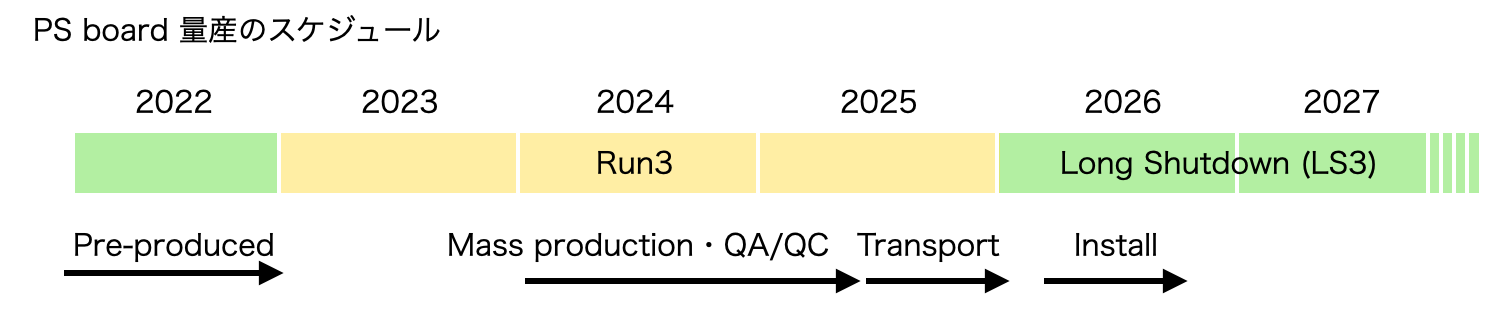
\includegraphics[width=16cm]{fig/QAQC/PSBschedule.png}
\caption[PS board量産のスケジュール]{PS board量産のスケジュール。PS boardはこれまでに第一試作機、第二試作機を通したシステム開発が完了している。2023年現在、プレ量産された各個体に対しての試験を進めている。2024年から1400枚の本量産が開始され2026年からATLAS実験室への設置が開始される。}
\label{PSBschedule}
\end{figure}

\newpage
\subsection{PS boardに搭載された素子}
\label{subsec_PSBelements}
QAQC試験ではエレクトロニクス上のすべての素子間の導通を網羅的に検証することが重要である。
PS boardに搭載されている素子やそれらの間をつなぐ配線を精査し、ハードウェアの試験に適したセットアップおよび試験内容を考案した。

図\ref{PSBconcept}にPS boardに搭載されている素子、各素子間の配線を示す。また、以下にPS board上に搭載されている各素子の役割と各素子間をつなぐ配線をまとめる。

\begin{figure} 
\centering
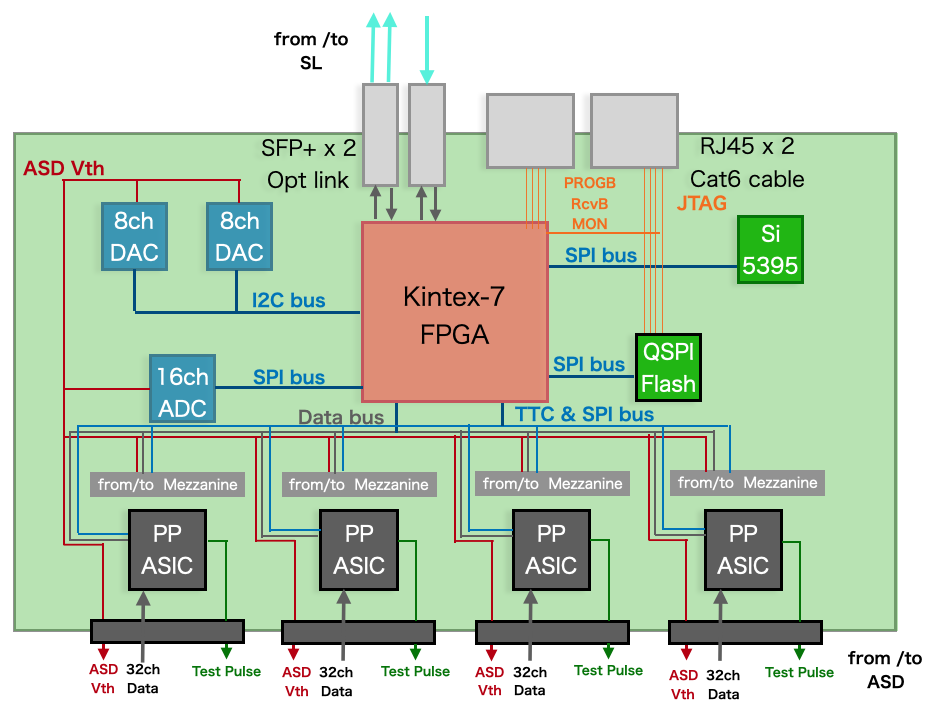
\includegraphics[width=16cm]{fig/QAQC/PSBoverall.png}
\caption[PS boardの全体像]{PS boardの全体像。PS boardに搭載されている素子とその間の配線を示す。PS boardはSLと3本の光ファイバーで接続され、高速シリアル通信を行う。PS board FPGAから送られるパラレル信号はSFP+モジュールで電気信号から光信号へと変換される。また、PS boardはJATHubと2本のCat-6ケーブルで接続される。1本はJTAG線と呼ばれ、JATHubからQSPIフラッシュメモリーにファームウェアを書き込むのに利用される。もう1本はRecovery/Monitor線と呼ばれ、JATHubからPS boardに自己修復不可能なSEUが発生した際のファームウェア再コンフィギュレーションのための信号が送られる。PS board FPGAとDACとは$I_{2}C$バスで接続され、ADC、Si5395、QSPI、PPASICとはSPIバスで接続される。DACからASDへはアナログの閾値電圧が供給され、ADCがそれをモニターする。PS board FPGAはPP ASICにTTC信号を送信し、ヒット信号を受信する。1つのPP ASICは2台のASDボードと接続されそれぞれから8チャンネル分のヒットデータを受信する。PP ASICからASDへテストパルスを発行する機構もある。}
\label{PSBconcept}
\end{figure}

\vskip0.5\baselineskip

\begin{enumerate}
    \item \texttt{SFP+ :} 電気信号と光信号の変換するモジュール。PS board FPGAは3本の光ファイバーを介してSLと通信する。2線は送信用に定義されており、1枚のPS boardが担当する256チャンネルのヒット信号をヒットの有無に関わらず送信する。1線は受信用に定義されており、コントロール信号を受け取る。コントロール信号にはTTC信号も含まれ、PS boardはシリアルデータから40 MHzのLHCバンチ交差クロックを再構成する。
    \vskip0.5\baselineskip

    \item \texttt{RJ45コネクター :} Cat-6ケーブルを接続するためのコネクター。JATHubとPS boardは2本のCat-6ケーブルで接続され、LVDS規格で通信する。1線はJTAG線として定義され、JATHubがJTAG4線をドライブすることでPS boardのQSPIフラッシュメモリーにファームウェアを書き込む。もう1線はRecovery/Monitor線として定義され、PS boardに自己修復不可能なSEUが発生した場合のリカバリー手続きと、PS board FPGAで再構成したLHCバンチ交差クロックのモニター用に使われる。
    \vskip0.5\baselineskip

    \item \texttt{QSPIフラッシュメモリー :} 電力供給を切ってもデータを保持し続ける不揮発性のメモリー。PS board FPGAとはSPIバスで接続される。PS boardではファームウェアや制御用パラメーターを保存するのに使われる。ファームウェアはJATHubがJTAG線をドライブすることで、PS board FPGAを経由して書き込まれる。制御用のパラメーターはSLがコントロール線に乗せてSPIプロトコルをビットバンギングし、PS board FPGAがそれを中継することで書き込まれる。PS board FPGAは自動でこれらのパラメーターを読み出し、PP ASICやDACへ自ら分配する (自立型制御機構)。
    \vskip0.5\baselineskip

    \item \texttt{PP ASIC :} 2台のASDから送られるデジタル信号をBCIDし、LHCバンチ交差クロックと同期させる。可変遅延回路における信号遅延の大きさや、陽子バンチ識別回路の有効ゲート幅などはASDごとに異なるパラメーターを設定する必要がある。これらのパラメーターは上述の自立型制御機構により、SLから設定され、PS board FGPAからSPIバスを通じて分配される。その他にもPS board FPGAはTTC信号やテストパルストリガー信号をPP ASICに供給する。PP ASICはPS board FPGAに16 チャンネル分のヒット信号を送信する。またPP ASICはASDにテストパルスを供給する。
    \vskip0.5\baselineskip            

    \item \texttt{DAC :} ASDのコンパレーターに閾値電圧を供給する。PS board FPGAとは$\mathrm{I_{2}C}$バスで接続される。ADCに印加する閾値電圧の極性や大きさなどのパラメーターは自立型制御機構により分配される。設定されたパラメーターはPS board FPGAの自立型監視機構により定期的に読み出され、SLに送信される。
    \vskip0.5\baselineskip

    \item  \texttt{ADC :} DACからASDに供給される閾値電圧をモニターする。PS board FPGAとはSPIバスで接続される。ADCの値は自立型監視機構により定期的に読み出され、SLに送信される。
    \vskip0.5\baselineskip

    \item \texttt{Si5395 :} PS board FPGAがシリアルデータから再構成したLHCバンチ交差クロックのジッターを低減し、FPGAやGTXトランシーバーへ分配する。PS board FPGAとはSPIバスで接続される。Si5395にはクロックのインプットポートの設定や、アウトプットクロックの周波数などいくつかの制御用パラメーターが存在するが、1434枚のPS boardで共通で、今後変更の予定もない。そこで、制御用パラメーターはQSPIフラッシュメモリーではなくFPGA内のBRAMに格納され、自立型制御機構のシークエンスの中で分配される。
    \vskip0.5\baselineskip

\end{enumerate}

\subsection{QAQC試験の設計}
\label{subsec_QAQCdesign}
\ref{subsec_PSBelements}節で述べたすべてのインターフェイスと素子を網羅的にテスト可能なセットアップとして、JATHubを利用する試験システムを考案した。図\ref{PSBtestdesign}にその概念図を示す。

\begin{figure} 
\centering
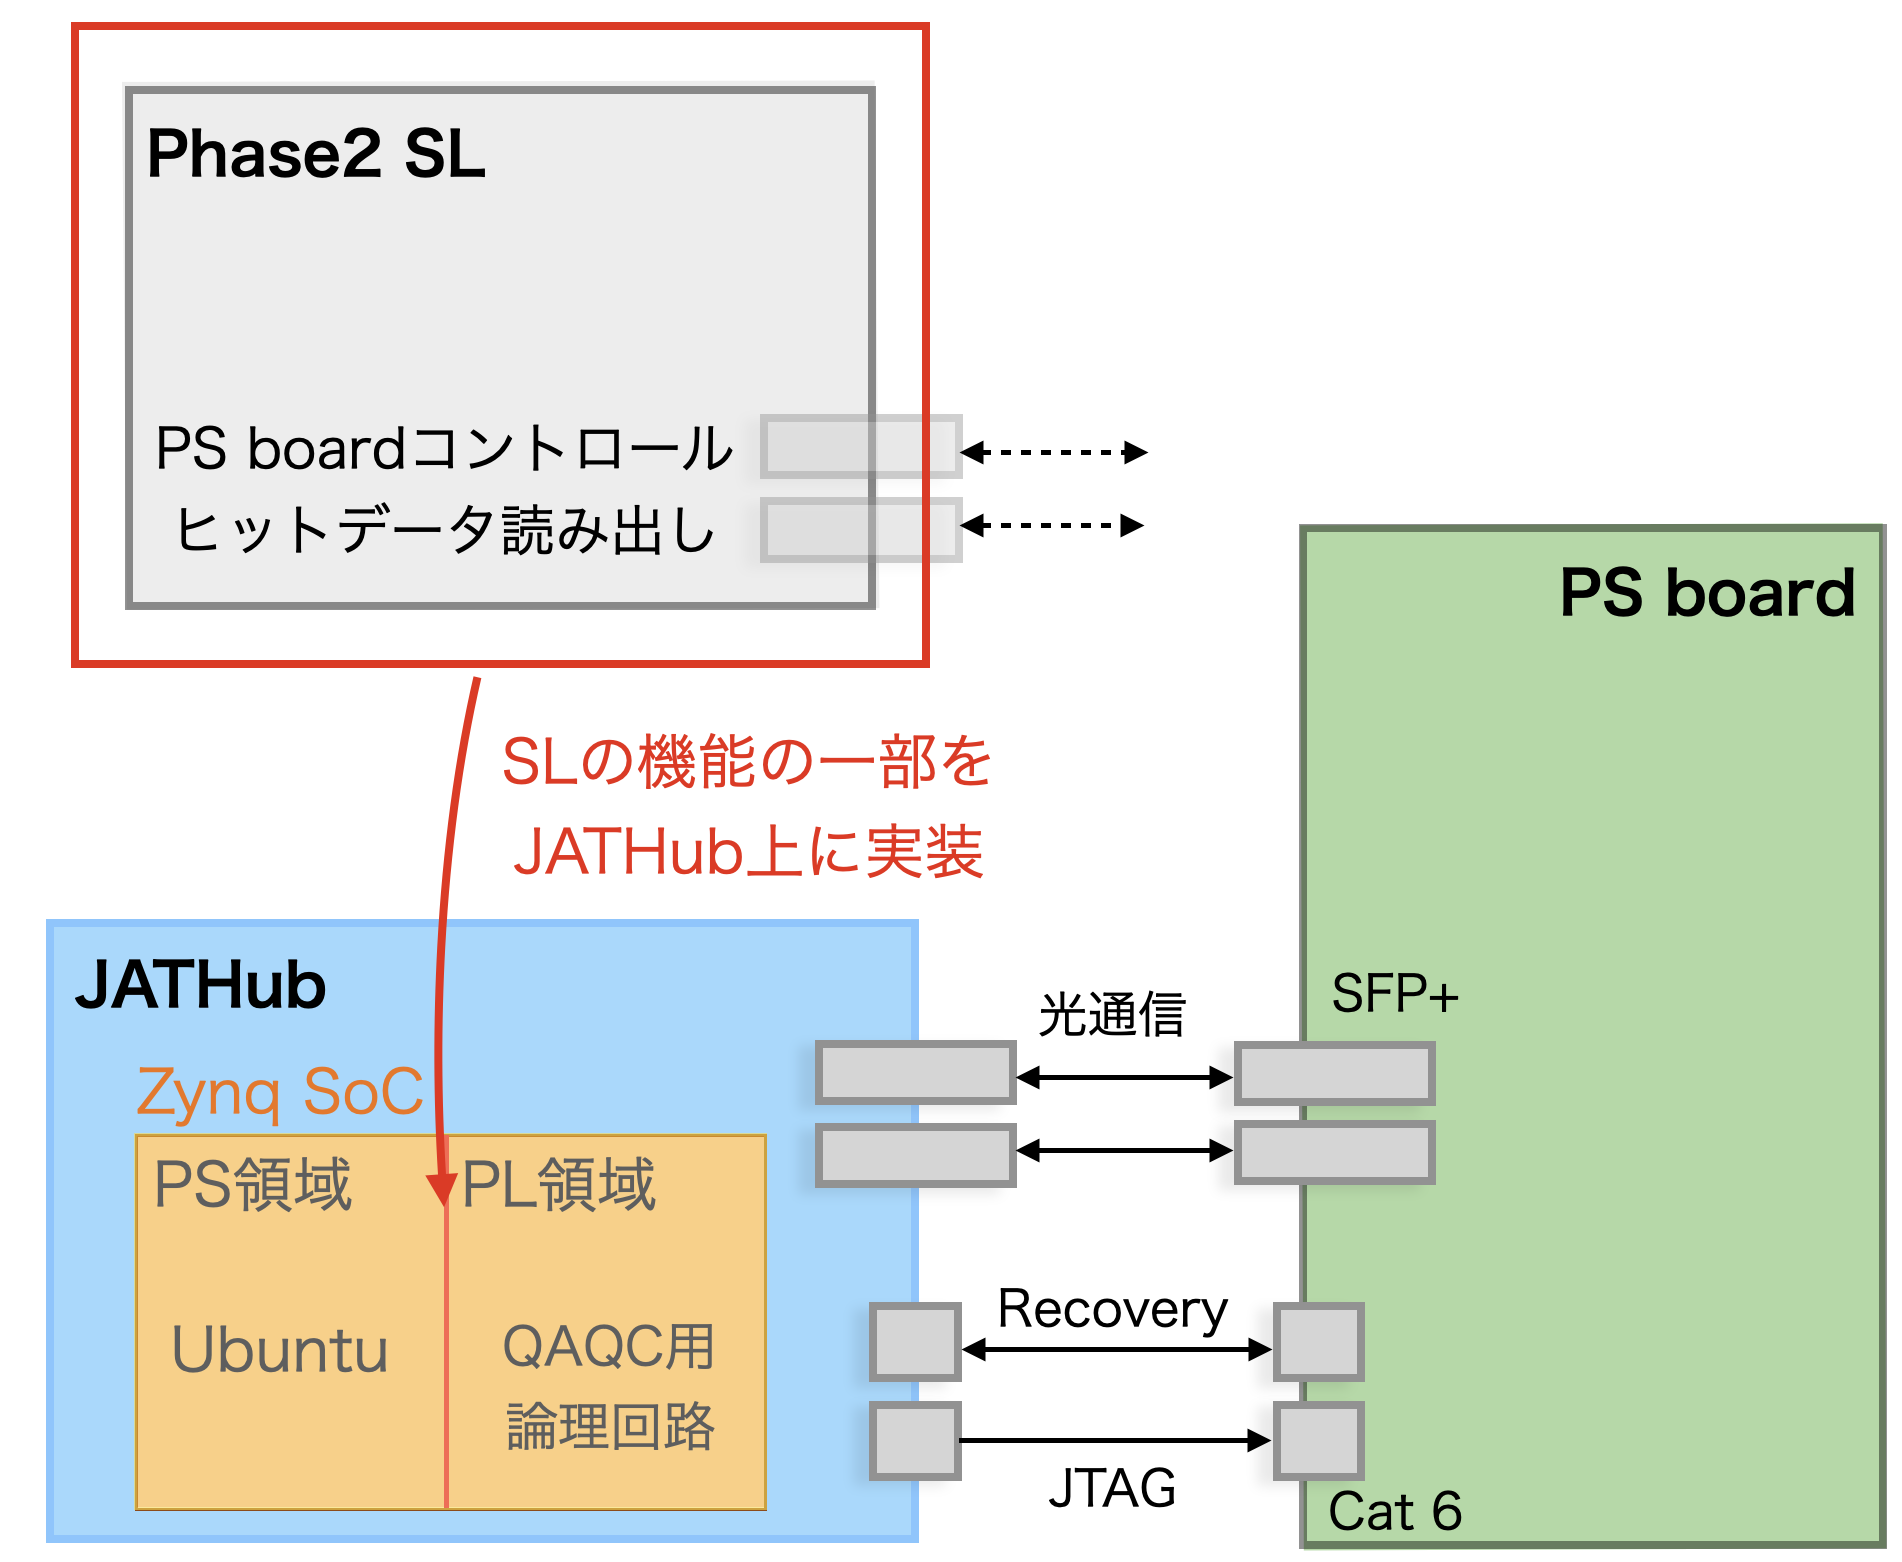
\includegraphics[width=16cm]{fig/QAQC/PSBtestdesign.png}
\caption[PS board QAQC試験セットアップの概念図]{PS board QAQC試験セットアップの概念図}
\label{PSBtestdesign}
\end{figure}

このシステムではPS boardの1台の試験にJATHub1台のみを利用する。JATHubとPS boardは2本のCat-6ケーブルと3本の光ファイバーで接続する。
このシステムのコンセプトは、SLが担うPS boardからヒットデータを受信する機能とコントロール信号を送信する機能をそのままJATHubに実装し、SLを用いることなくPS boardの機能を網羅的に試験することである。
SLを駆動するためにはATCAクレートが必要で、それに伴った大掛かりなセットアップが必要となる。その点JATHubはデスクトップで給電することも可能であり、場所を選ばない汎用的な試験システムを実現できる。QAQC試験のマスターとして動作させるJATHubを以降ではQAQC用JATHubと呼ぶ。
PS boardには試験用のファームウェアなどは用意せず、本番用のファームウェアを用いる。これによりハードウェアの検査に加えて、PS board FPGAで使われるファームウェアの検証も同時に行うことができる。
JATHubのメインドライバーであるZynq SoCのPS領域にはUbuntuを起動し、試験のマスターとして動作させる。試験ではローカルのPCからイーサーネット経由でUbuntuにアクセスし、アプリケーションを実行することで試験用信号の発出や、試験用データの読み出しを行う。Ubuntuは汎用的なOSであり、既存のソフトウェアを用いてネットワーク、webサーバー等の設定を行ったり、コンパイラをインストールすることでUbuntu上で直接アプリケーションを開発することができるため、簡単に開発を進めることができる。
FPGA部分であるPL領域には試験用に新しくファームウェアを開発する。
先行研究で開発された、Cat-6ケーブルを介してPS boardを制御する機能 (JTAG線をドライブする機能、リカバリー手続き、クロックの位相測定) に加えて、光ファイバーを介してPS boardを制御する機能 (GTXトランシーバー、コントロール信号の送信、ヒットデータ読み出し) も実装することで、JATHub1台でPS boardの有する機能を網羅的に試験することができる。
QAQC用JATHubのファームウェア開発にあたり、\ref{subsec_PSBelements}節で挙げたPS board上のすべての素子とその間の導通を検証できる必要十分な試験として、ASDテストパルス試験とJTAG/Recovery/Clock monitor試験をベンチマークとして設定する。以下にそれぞれの試験の概要と手順を示す。

\subsubsection{ASDテストパルス試験}
\label{subsubsec_testpulse}
\vskip0.5\baselineskip

ASDテストパルスは、PP ASICからASDに送られる試験用の電荷であり、SLからASDまでのコントロールパスおよびデータパスのデバッグに使用される。図\ref{PSBasdtp}にその概要を示す。高輝度LHC-ATLAS実験のTGCシステムでは、CTPから生成されたTTC信号はSLを中継して各フロントエンドエレクトロニクスに分配される。テストパルスの駆動を司るテストパルストリガー信号(TPT)も同様のパスで、PS board FPGA、PP ASICへと伝達される。PP ASIC内のテストパルスジェネレーター回路 (図\ref{PSBtpg}) はTPT信号を受信すると、参照クロックである40 MHzクロックの立ち上がりと同期した差動の矩形波をASDに送信する。テストパルスの時間幅や波高はPS board FGPAから設定することができる。テストパルスはASD、PP ASIC、PS board FPGAによる処理を経て、ヒット信号としてSLに送信される。SLで期待したタイミングにヒット信号得られることを確認することで、ASDからSLまでのトリガーパスにハードウェアの不具合がないこと、およびFixed latencyでのデータ処理を実現できていることを確かめることができる。
\vskip0.5\baselineskip

\begin{figure} 
\centering
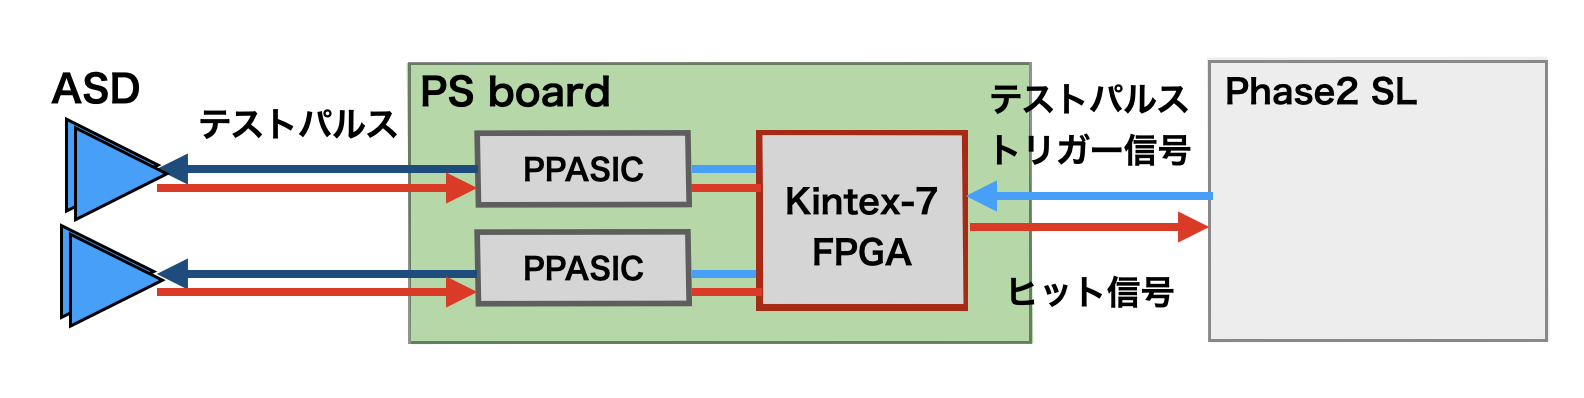
\includegraphics[width=16cm]{fig/QAQC/PSBasdtp.png}
\caption[ASDテストパルスの概念図]{ASDテストパルス機構の概念図。SLを起点にテストパルストリガー信号が駆動され、PS board FPGAを経由してPPASICに届けられる。PPASIC内のテストパルスジェネレーターはテストパルストリガー信号をトリガーに参照クロックの立ち上がりと同期した試験電荷をASDに送る。ASDで閾値電圧を信号はデジタル信号へ変換され、PPASIC、PS board FPGA、SLへとヒット信号が伝搬される。}
\label{PSBasdtp}
\end{figure}

\begin{figure} 
    \centering
    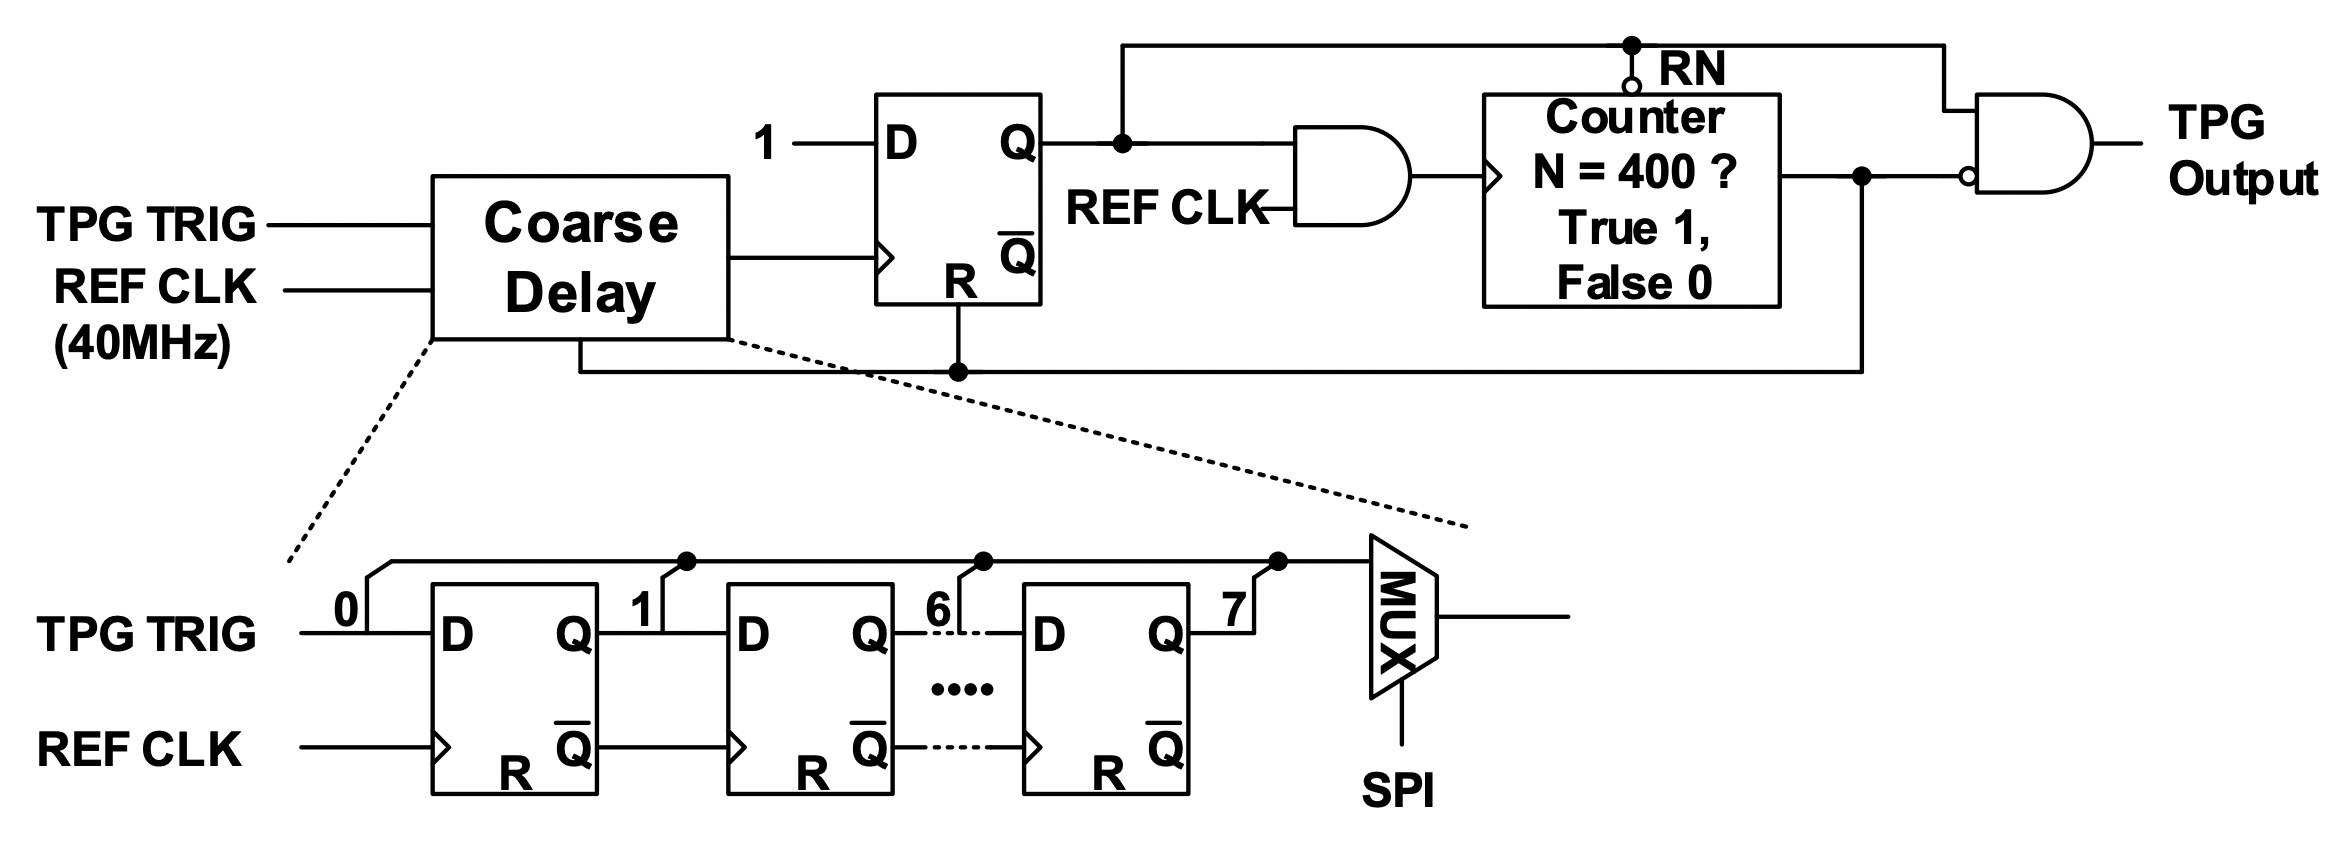
\includegraphics[width=16cm]{fig/QAQC/PSBtpg.png}
    \caption[テストパルスジェネレーターの回路図]{テストパルスジェネレーターの回路図。PS board FPGAからTRIG信号を受け取り、参照クロックである40 MHzクロックの立ち上がりに同期してASDに対して差動の矩形波を送信する。矩形波の幅や高さはFPGAから設定可能なパラメーターである。}
    \label{PSBtpg}
\end{figure}

図\ref{QAQCasdtp}に示すようにPS board QAQC試験ではQAQC用JATHubが試験のマスターとして機能し、PS boardの制御、テストパルストリガーの駆動、およびヒットデータの読み出しを行う。Zynq SoCのPL領域にPS board制御および読み出しのための回路を実装し、Ubuntu上のアプリケーションを起点にTPTの発行およびヒットデータ読み出しを行う。Ubuntuから読み出されたヒットデータは、ローカルのSDカード上にテキストファイルとして保存され、Ubuntu上そのまま解析が行われる。以下に試験の手順を示す。

\begin{figure} 
\centering
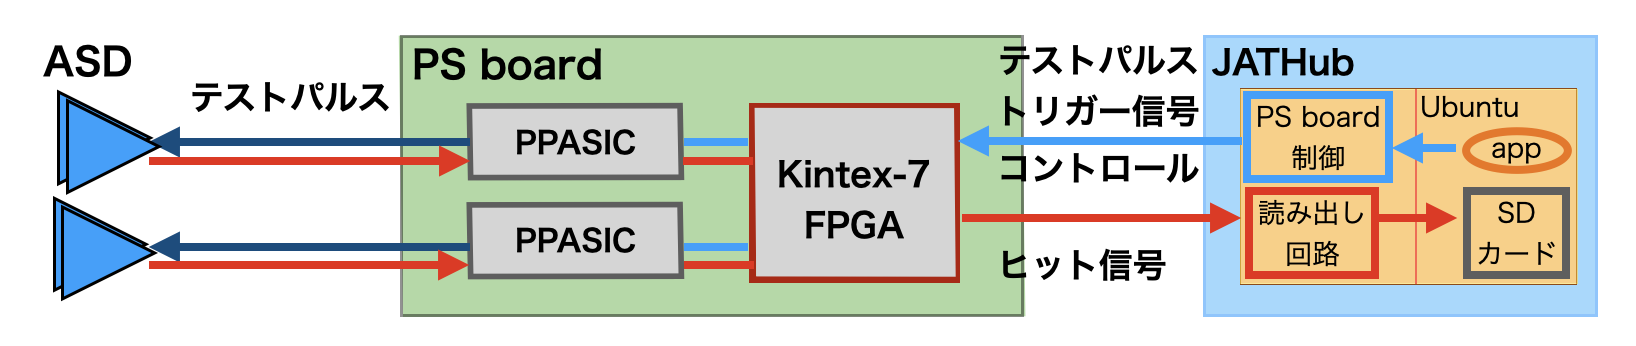
\includegraphics[width=16cm]{fig/QAQC/QAQCasdtp.png}
\caption[QAQC用JATHubを用いたASDテストパルス試験]{QAQC用JATHubを用いたASDテストパルス試験。QAQC用JATHubが試験のマスターとして、PS boardの制御、テストパルストリガーの駆動およびヒットデータの読み出しを行う。Zynq SoCのPL領域にPS board制御および読み出しのための回路を実装し、Ubuntu上のアプリケーションを起点に動作する。読み出し回路によりUbuntuに読み出されたヒットデータはローカルのSDカード上にテキストファイルとして保存する。}
\label{QAQCasdtp}
\end{figure}

\begin{enumerate}
    \item QAQC用JATHubをコントロールマスターとしてUbuntu上のアプリケーションを起点にPS boardに制御パラメーターを設定する。コントロール線を利用してSPIバスをビットバンギングすることで、PS board上のQSPIフラッシュメモリーに制御パラメーターを書き込む。その後、PS boardの自立型制御を再び走らせることでパラメーターをDAC、PP ASICに分配する。PP ASICの制御パラメーターとしては具体的に、ヒット信号遅延、有効ゲート幅、テストパルスの極性、テストパルスの波高、テストバルスの時間幅などがある。
    \vskip0.5\baselineskip

    \item QAQC用JATHubからコントロール信号に乗せてTPTを発行する。それに同期して、決まったレイテンシー後にL1A信号も発行する。これによりFixed Latencyでのデータ読み出しを実現する。
    TPTを発行してからヒット信号が帰ってくるまでのレイテンシーは試験セットアップ (シグナルケーブルや光ファイバーの長さなど) に依存するため、あらかじめセットアップに適した値を測定しておく。そのレイテンシーに合わせてL1 Bufferの深さを調整することで、TPTに対する応答に該当するBCのヒットデータを選択的に読み出すことができる。
    \vskip0.5\baselineskip

    \item TPTの発行とデータ読み出しをn回繰り返し、読み出したデータにヒットが入っていた割合をefficiencyとして評価する。コントロールパスおよびトリガーパスがFixed latencyで安定して動作している場合、efficiencyは100\%になる。
    \vskip0.5\baselineskip

\end{enumerate}

ASDテストパルス試験によって検証できる素子と素子間の導通を図\ref{QAQCasdtpelements}に示す。ASDテストパルスを期待通り動作させるにはPP ASIC、DAC、Si5395に適したパラーメーターを分配し、ASD、PP ASIC、PS board FPGA、光リンクが同期して動作する必要がある。この試験により赤色で示した領域を検証することができる。
\vskip0.5\baselineskip

\begin{figure} 
\centering
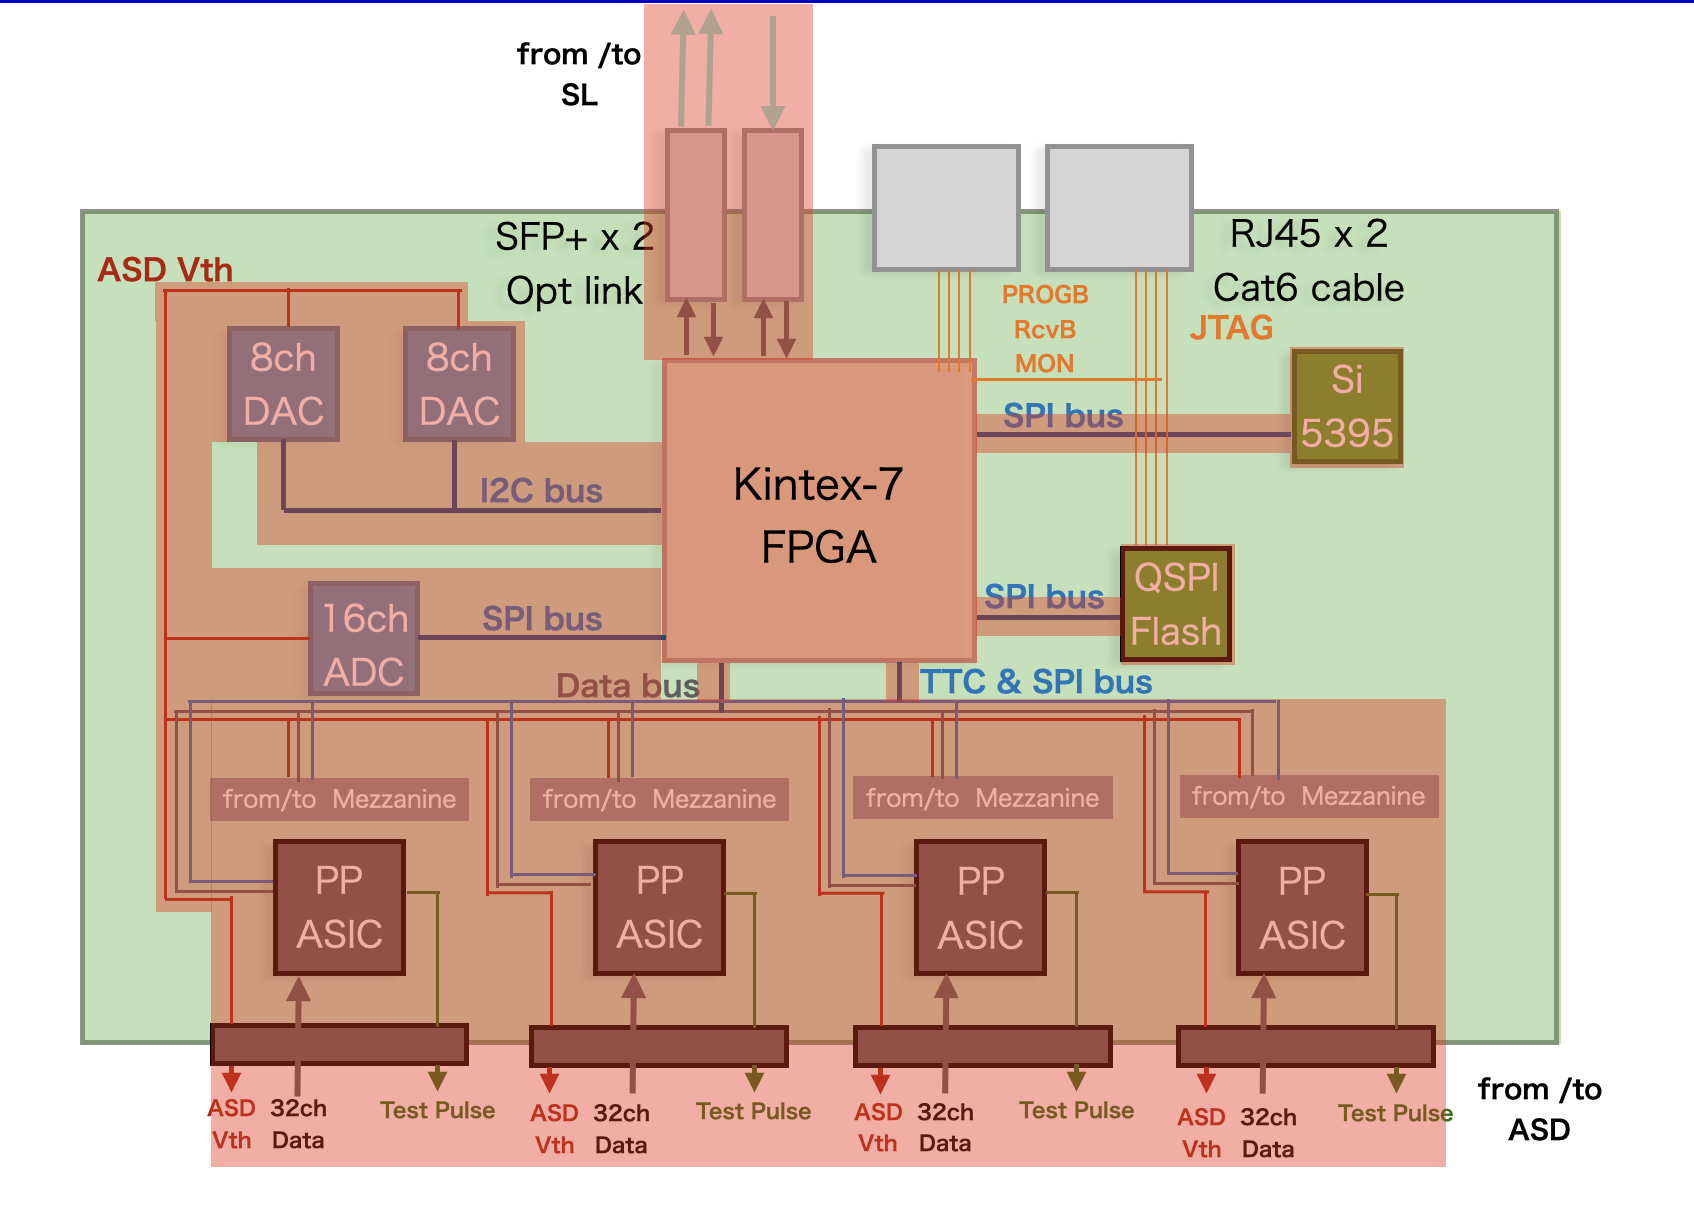
\includegraphics[width=16cm]{fig/QAQC/QAQCasdtpelements.png}
\caption[ASDテストパルス試験で検証できる素子]{ASDテストパルス試験で検証することができる素子、素子間の配線を赤枠で示す。}
\label{QAQCasdtpelements}
\end{figure}

\subsubsection{JTAG/Recovery/Clock試験}
\vskip0.5\baselineskip

\label{subsubsec_jtag}
JATHubがPS boardに対して行うJTAG線を介したファームウェアの書き込み、リカバリー手続き、クロック位相測定が動作することを試験する。以下に各試験の概要を示す。

\paragraph{JTAG試験}\par
JTAG試験はZynqに起動したOSからJTAG線をドライブして、FPGAやQSPIフラッシュメモリーにファームウェアを書き込むことができるか試験する。これにはSerial Vector Format player (SVF) と呼ばれるアプリケーションを用いる。
SVF playerはSVFファイルと呼ばれる、JTAG4線をドライブするパターンを記述したACSII (テキスト) ファイルを読み込み、PS-PL間チップ通信を利用してJTAG線を操作する。SVFファイルはXilinx社が提供するFPGA開発用ソフトウェアVivadoで作成することができ、QAQC用JATHub内のSDカードに置かれる。
\vskip0.5\baselineskip

\paragraph{リカバリー試験}\par
%図作る
リカバリー試験はPS boardに自己修復不可能なSEUが発生したことを仮定して、救難信号を出力させ、QAQC用JATHubから再コンフィギュレーションできることを確かめる試験である。PS boardにレジスタ操作によりマニュアルで救難信号 (RcvB線) を出させる仕掛けを実装し、一連のリカバリー手続が動作するか試験する。
\vskip0.5\baselineskip

\paragraph{クロック試験位相測定}\par
クロック位相測定試験では、MON線で送られるPS boardで再構成したLHCバンチ交差クロックの位相を測定することができるか試験する。試験システムの概念図を図\ref{JATHubclockmeasure}\cite{mt_atanaka}に示す。JATHub内の水晶発振器から生成した40 MHzクロックを参照クロックとして、その立ち上がりのタイミングでLHCバンチ交差クロックをラッチする。参照クロックを1/56 ns刻みでスキャンしながら、ラッチを繰り返すことでLHCバンチクロックの位相を測定することができる。
\vskip0.5\baselineskip

\begin{figure} 
    \centering
    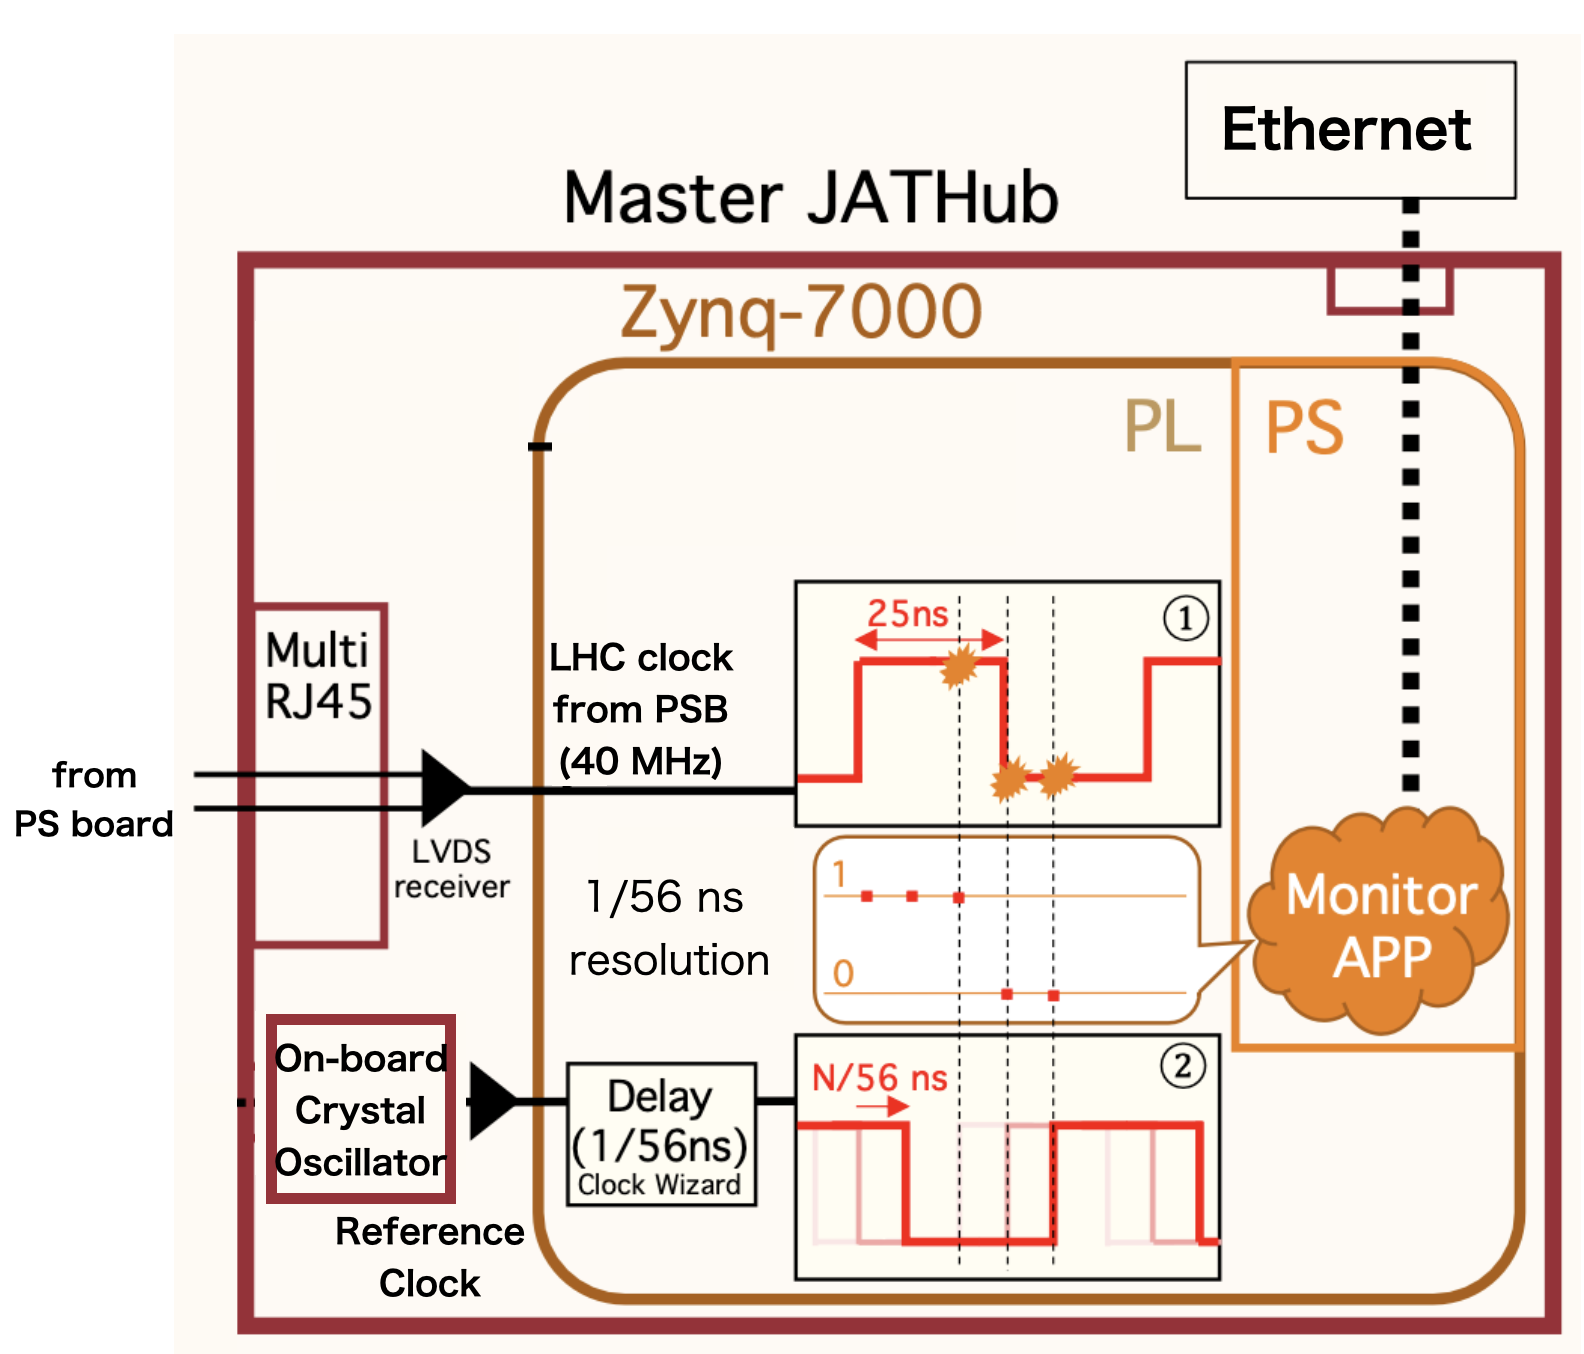
\includegraphics[width=16cm]{fig/QAQC/JATHubclockmasurement.png}
    \caption[JATHubによるクロック位相測定の概念図]{JATHubによるクロック位相測定の概念図\cite{mt_atanaka}}
    \label{JATHubclockmeasure}
\end{figure}    

\section{JATHubを用いた機能実装}
本節では\ref{subsec_QAQCdesign}節で考案した試験を実現するために開発したQAQC用JATHubの機能実装について述べる。

\subsection{システムの概要とインフラの実装}
\label{subsec_infra}
試験セットアップにおけるシステムの概要とシステムをまたぐインターフェイスについて述べる。
図\ref{JAThubinfra}にセットアップの概念図を示す。QAQC試験におけるコントール信号は、ローカルPCを起点にPS、PL、PS boardの順に送られる。
ASDテストパルスなどのデータパスは、PS board、PL、PS、ローカルPCの順にデータを伝搬する。
PSにはUbuntuが起動しており、ローカルPCとUbuntuはネットワーク経由で通信を行う。
PSとPLの通信はXilinx社が提供するAXIプロトコルに従って行う。
PLからPSへのデータを読み出しは、高速かつ安定したDAQを実現するために開発したAXI GPIOを応用した自作調停回路を利用する。
PLとPS boardの通信には光通信が使われ、PL領域に固定位相のGTXトランシーバーを実装した。
以下に各システムとインターパスの実装について詳しく説明する。

\begin{figure} 
\centering
\includegraphics[width=16cm]{fig/QAQC/JAThubinfra.png}
\caption[QAQC用JATHubのシステム全体像]{QAQC用JATHubのシステム全体像}
\label{JAThubinfra}
\end{figure}

\subsubsection{Zynq PS領域におけるUbuntuの起動}
\label{subsubsec_ubuntu}
\vskip0.5\baselineskip
Zynq SoCのPS領域には標準的なLinux OSであるUbuntuを起動する。Ubuntuは汎用性と拡張性に富んだOSでネットワークの設定やQAQC用JATHub内部でのアプリケーション開発を容易に行うことができる。\par

Zynq組み込みデザインの開発には64bit Ubuntu 18.04.6を使用した。Xilinx社が提供する”Vivado 2020.2”を利用してZynq PL部に構築する自作論理回路の開発やPS部のIO設計を行った。Vivadoで開発した論理回路は最終的にBitstreamファイルと呼ばれるバイナリーファイルとして出力される。Zynq PS 部で走るLinuxの設定はXilinx社が提供するクロスコンパイラー”petalinux 2020.2”を利用した。PetalinuxではVivadoで生成したHDFを元にデバイスツリーやRoot File System(rootfs)を設定することで、Zynqの起動に必要なブートファイルを作成することができる。\par
QAQC用JATHubではUbuntuの起動にSDカードを利用する。SDカードには2つのパーティション\footnote{ブートファイル用のパーティションはfat32、Ubuntuのrootfs用のパーティションはext4で展開する。}を用意し、Zynqの起動に必要なブートファイルとUbuntuのルートファイルシステムをそれぞれ展開する。図\ref{JATHubboot}にZynq上でのUbuntu起動の流れを示す\cite{mt_okazaki}。JATHubに電源を投入すると以下のシークエンスでUbuntuが起動する。

\begin{figure} 
\centering
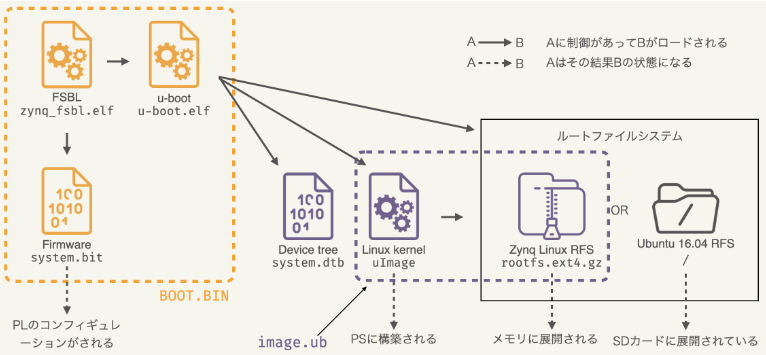
\includegraphics[width=16cm]{fig/QAQC/JATHubboot.png}
\caption[Ubuntuの起動シークエンス]{Ubuntuの起動シークエンス}
\label{JATHubboot}
\end{figure}

\begin{enumerate}
    \item First Stage Boot Loader(FSBL)がロードされる
    \item ファームウェアのビットストリームがSoCのPL部に書き込まれる
    \item LinuxカーネルやOSを起動するためのブートローダーであるu-bootがロードされ、制御が移行される。
    \item u-boot 制御下でデバイスのハードウェア情報を記述したデバイスツリーがロードされる。
    \item u-boot 制御下でLinux kernelがロードされPS部に構築される。
    \item 制御がLinuxカーネルに移行されLinuxが起動する。
\end{enumerate}

\subsubsection{LANケーブル経由のネットワーク通信}
\label{subsubsec_network}
\vskip0.5\baselineskip
QAQC試験で用いるJATHub試作1号機は図\ref{JATHub_ether}に示す2通りの方法でEthernet通信を行うことができる。1つ目はLANケーブルを使用するもので、回路上の搭載されたPHY chip (Micrel PHY Chip) を利用して、Ethernet信号をCPUが扱える信号に変換する。2つ目は光ケーブルを用いる方法で、GTXトランシーバーで受けた光信号を1000BASE X PCS/PMAと呼ばれるIPブロックを利用して処理する。両者の切り替えはVivado上でPS部のconfigurationを変更することで簡単に行うことがでいる。QAQC用JATHubでは3本の光ファイバーはPS board 通信に利用するため、LANケーブル経由のネットワーク接続を行う。

\begin{figure} 
\centering
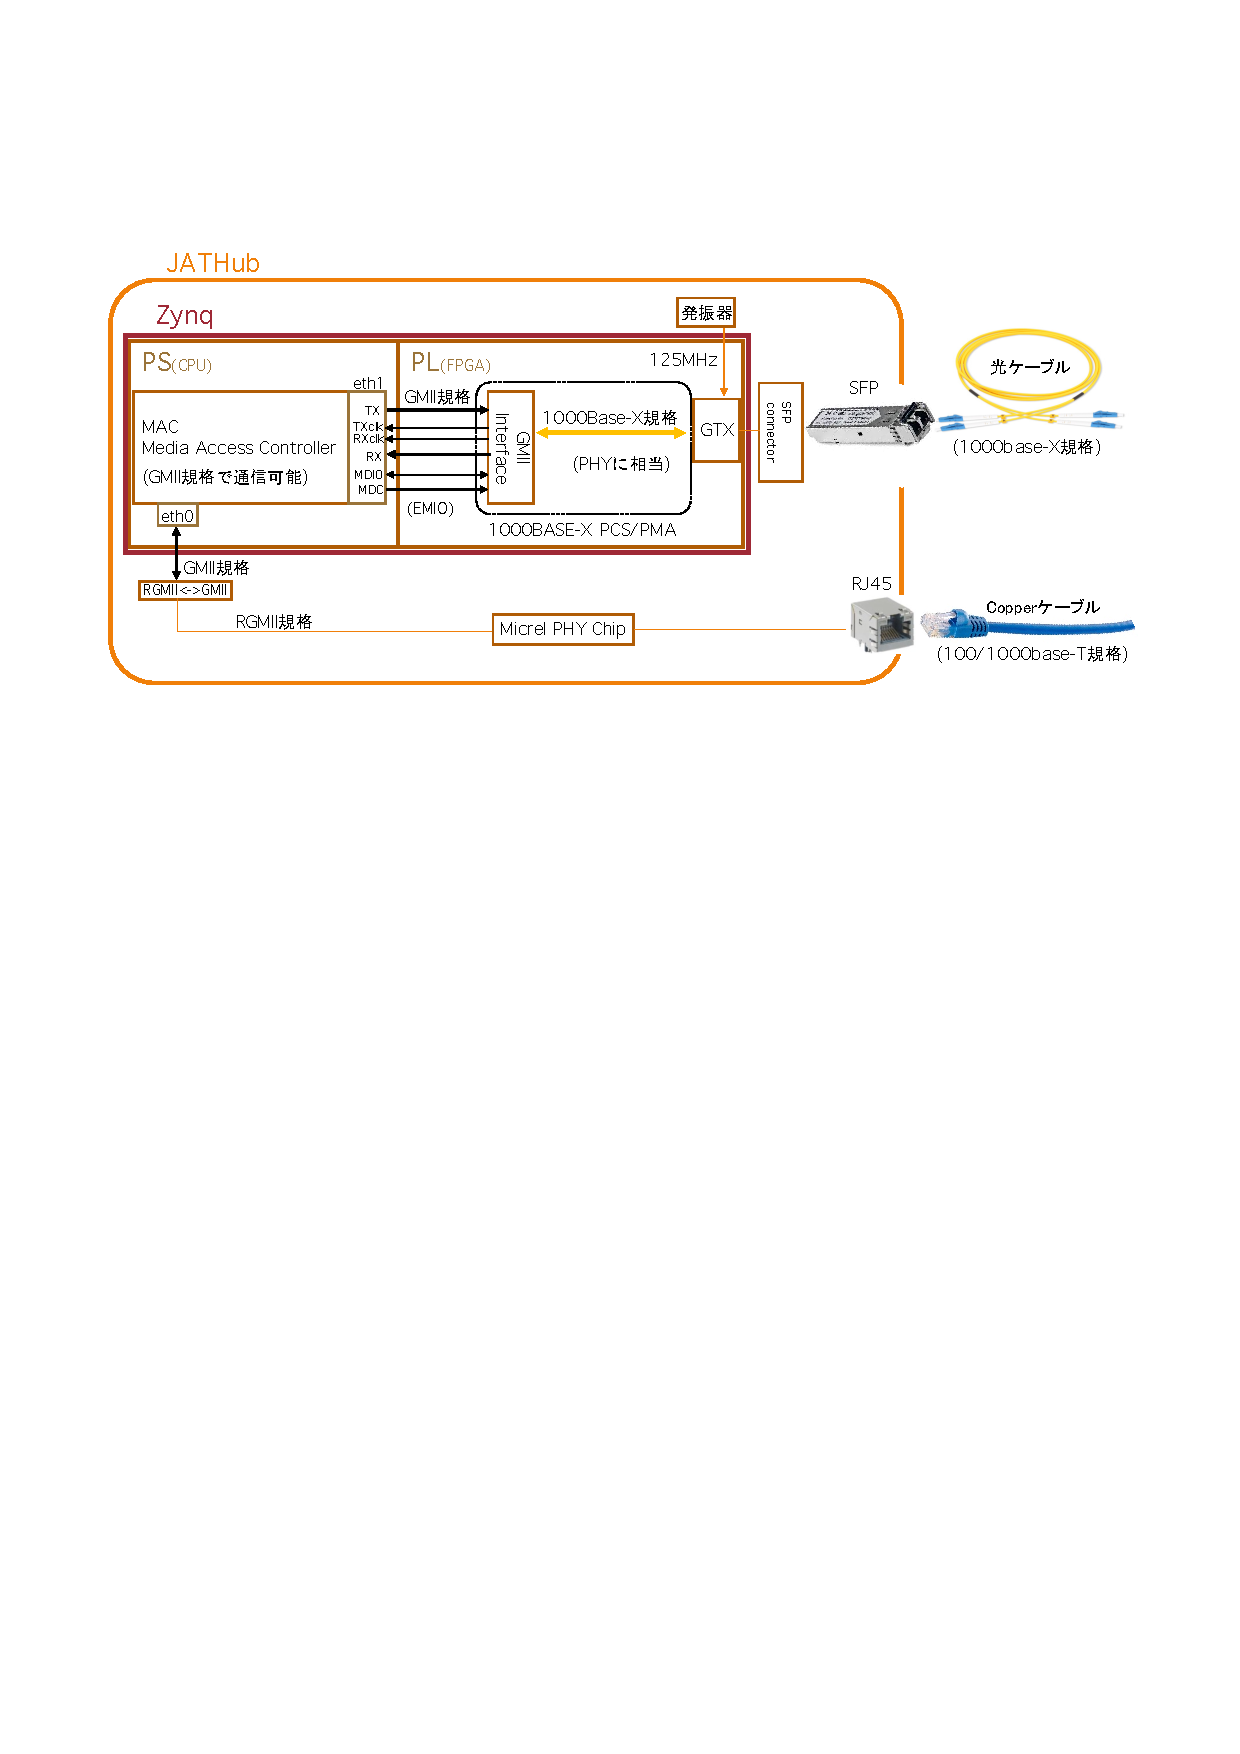
\includegraphics[width=16cm]{fig/QAQC/JATHub_ether.pdf}
\caption[光Ethernet通信の仕組み]{光Ethernet通信の仕組み\cite{mt_atanaka}}
\label{JATHub_ether}
\end{figure}


\subsubsection{AXI GPIOを用いたPSからPLへのアクセス}
\label{subsubsec_axi}
\vskip0.5\baselineskip
PS領域からPL領域への通信は統一的にAXI General Purpose Input Output (GPIO)を介して行う。AXI GPIOによって接続されたPLのレジスタには固有の物理アドレスが割り当てられる。割り当てられれた物理アドレスの例を図\ref{JATHuaddress}に示す。このアドレスはVivadoのAddress Mapで確認することができ、Address Editorにてユーザーが自由に変更することができる。
PS領域からAXI GPIOレジスタへは少なくとも2通りの方法でアクセスすることができる。1つはUbuntuルートファイルシステム内の/dev/memが提供するキャラクターデバイスをアプリケーションから直接開く方法である。/dev/memを介したアクセスではUbuntuが扱うすべての物理アドレスに制限なくアクセスすることができるため、簡単に使用できる。一方、カーネル動作に必要なレジスタにも意図せずアクセスする危険があるため、カーネルを壊す危険性がある。2つ目の方法は特定のAXI GPIOレジスタをUser space I/O (UIO) としてデバイスツリーに登録し、アプリケーションからUIOドライバーを介してアクセスする方法である。この方法ではUIOに登録したアドレス以外へのアクセスは禁止されるためカーネルを壊す危険性がなくなる。また割り込み処理ができるという利点もある。
コントロールパスにおいてはより実装が簡単な/dev/memを直接用いる方法をとっている。
\vskip0.5\baselineskip

\begin{figure} 
\centering
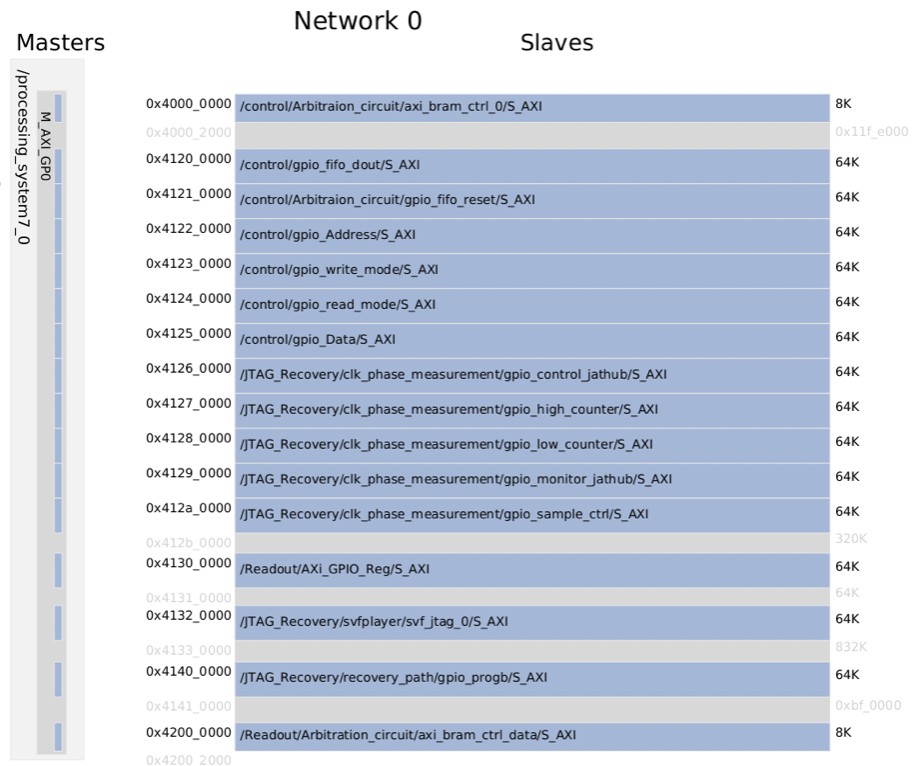
\includegraphics[width=10cm]{fig/QAQC/JATHubaddress.png}
\caption[アドレスマップ]{JAThub PL領域に割り当てられたアドレスマップ。各AXI GPIOレジスタには固有の物理アドレスが割り当てられる。}
\label{JATHuaddress}
\end{figure}

\subsubsection{固定位相光シリアル通信のためのGTXトランシーバーの実装}
\vskip0.5\baselineskip
\label{subsubsec_gtx}
\ref{subsec_PSBelements}節で述べたようにSLとPS boardの間では光ファイバーを介した固定位相のクロック分配が行われる。LHCバンチ交差クロックとPS baordで再構成されるクロックの位相関係が、電源の再投入や光リンクのリセットで変化しないことは、PP ASICで適切なBCIDをするのに必要不可欠な要請である。PS boardのこの機能を検証するため、QAQC用JATHubを用いたASDテストパルス試験においても固定位相でのDAQが実現できていることを確認する。そこで先行研究\cite{mt_aoki}で開発された、固定位相でのクロック再構成を可能にする、特別なGTXトランシーバーを本システムにも組み込んだ。図\ref{JATHubgtx}に実装したGTXトランシーバーの概要を示す。
\vskip0.5\baselineskip

\begin{figure} 
\centering
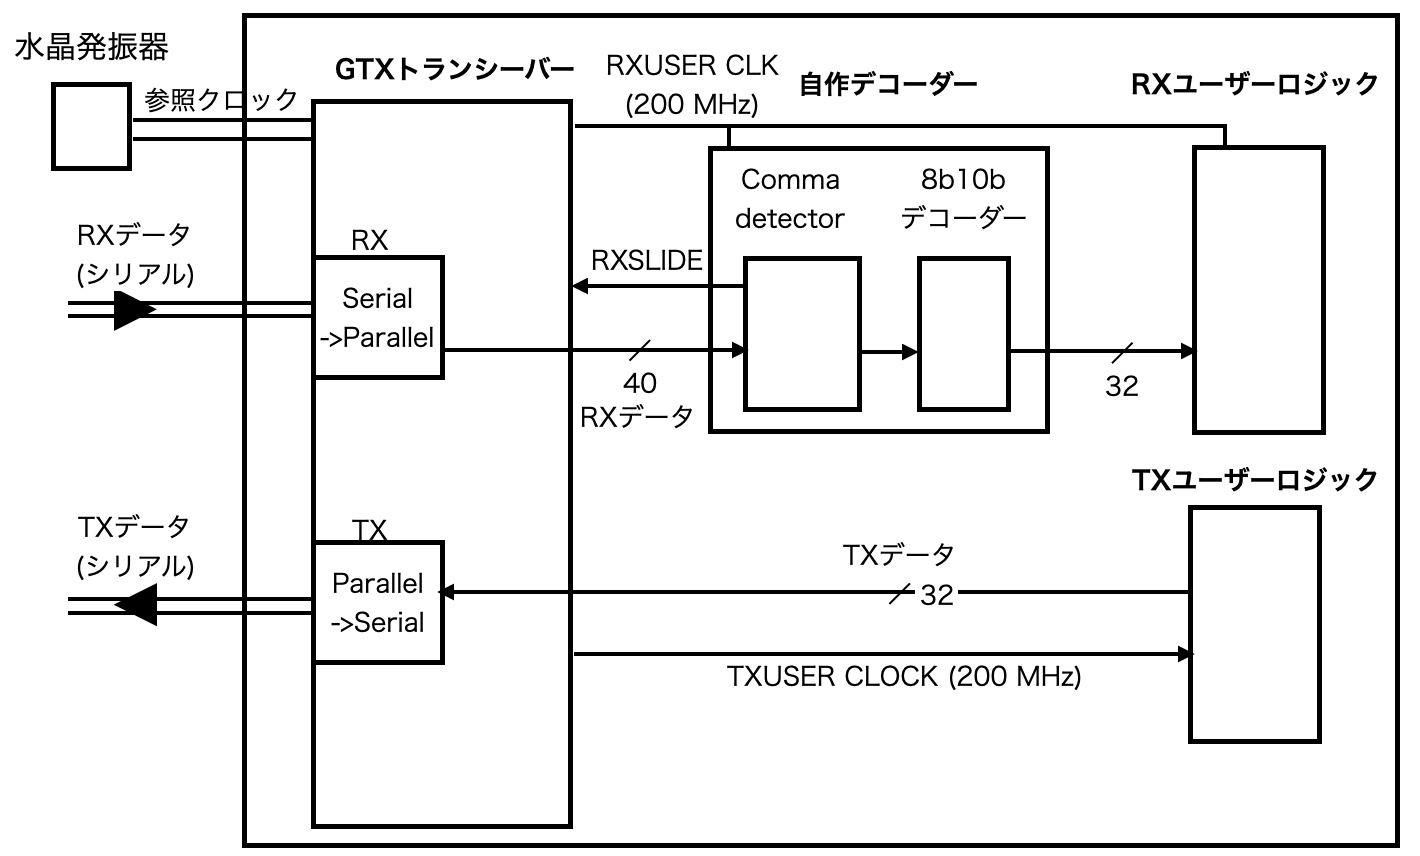
\includegraphics[width=16cm]{fig/QAQC/JATHubgtx.png}
\caption[QAQC用JATHubにおけるGTXトランシーバーの概要]{QAQC用JATHubにおけるGTXトランシーバーの概要}
\label{JATHubgtx}
\end{figure}


\paragraph{TXロジック} \par
GTXトランシーバーはJATHub内部の水晶発振器から生成される160 MHzクロック\footnote{正確にはLHCバンチ交差クロック40.079 MHzの4倍に相当する160.316 MHz。}を参照クロックとして利用する。\ref{subsec_PSBelements}節で述べたようにQAQC用JATHubとPS boardは8 Gbpsの高速光通信を行う。TXロジックでは160 MHzの参照クロックを200 MHzに分周したものをTXユーザークロックとして利用する。200 MHzおきに32bitのパラレルデータ(1ワードと呼ぶ)をGTXトランシーバーに送信し、GTXトランシーバー内で8b/10bのプロトコルで40 bitのパラレルデータへとエンコードした後、シリアルデータへと変換する。生成されたシリアルデータは参照クロックをGTXトランシーバー内のPhase Locked Loop(PLL)で冪倍して得られる4 Gbpsのクロックに乗せて送信される。
\vskip0.5\baselineskip

\paragraph{RXロジック} \par
RXロジックで固定位相のクロック再構成を実現するために重要な役割を果たすのが、RX Clock Data Recovery機構(CDR)とcomma detectorである。CDR機構とは受信したシリアルデータの立ち上がりまたは立ち下がりのタイミングに同期してクロックを再構成する機能で、受信データと位相関係を固定してクロックを再構成することができる。CDRで再構成された4 GHzクロックは1/20に分周され、200 MHzのRXユーザークロックが作られるのだが、その過程で合計20種類の位相の不確定性が生じる。この中から特定の1つの位相を決めるために用意されているのがComma detectorである。commaデータとは送信側と受信側の間で事前に取り決められた10 bitの予約語で、本システムでは40 MHzに1回送信するよう決める。comma detectorはcommaデータが下位10 bitにくるまでシリアルデータをシフトする機能で(図\ref{JATHubcomma})、これにより40 MHzで送信される200 bitのシリアルデータから再構成されるクロックの位相を一意に定めることができる。

\begin{figure} 
\centering
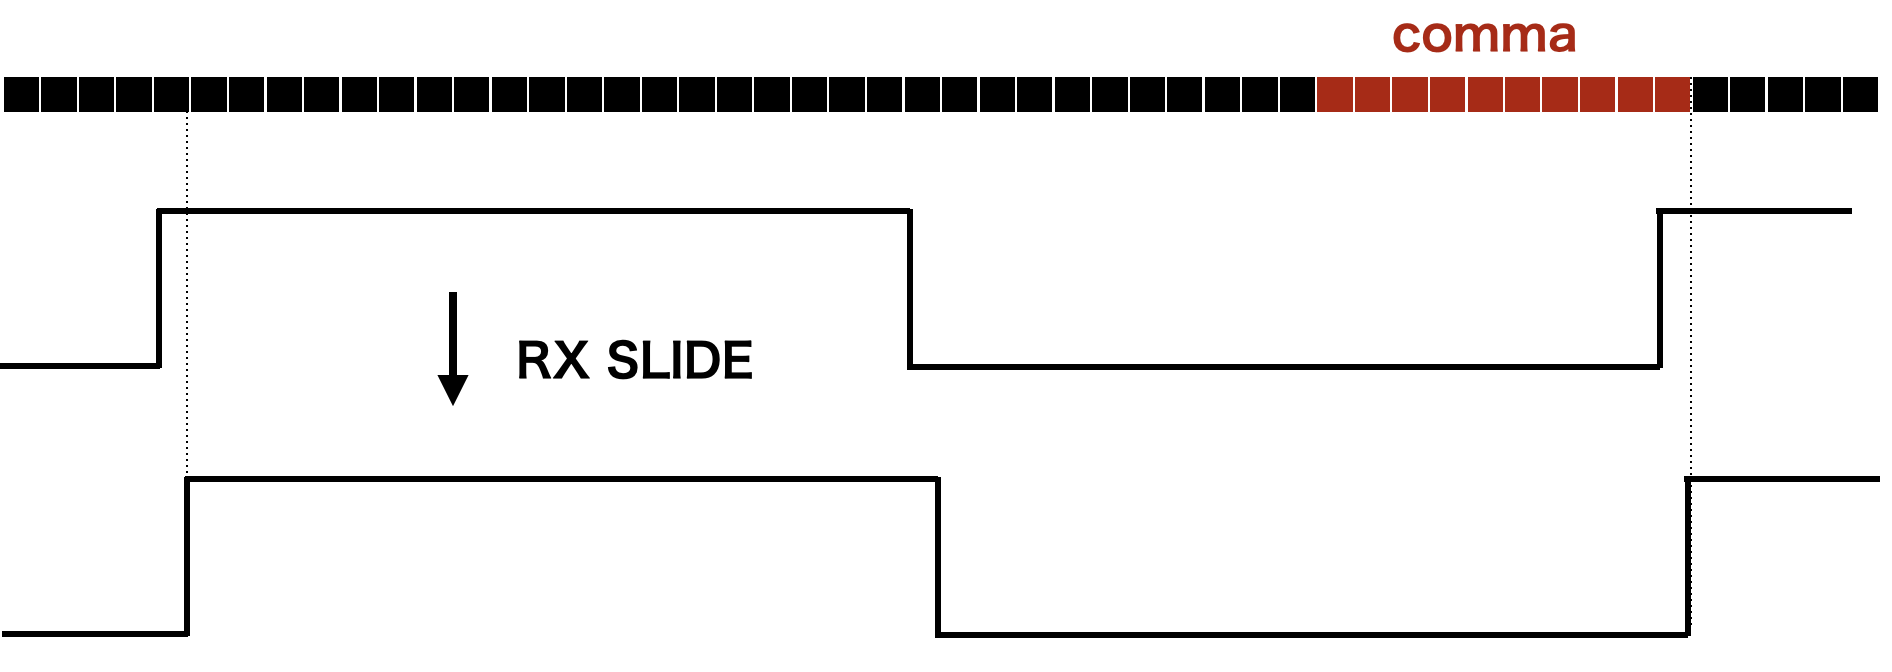
\includegraphics[width=16cm]{fig/QAQC/JATHubcomma.png}
\caption[comma detectorの概要]{comma detectorの概要}
\label{JATHubcomma}
\end{figure}
\vskip0.5\baselineskip


\subsubsection{PLからPSへのデータ読み出しシステムの設計}
\vskip0.5\baselineskip
\label{subsubsec_readout}

FPGA内での信号の遷移は$\mathcal{O}(10)$ MHzの高速クロックを基準クロックとして行われる。一般にプロセッサーを$\mathcal{O}(ns)$で制御し、FPGAと同期してデータを読み出すことは困難である。そこでQAQC用JATHubでは異なる速度で動作する2つのプロセス間のデータ転送に利用される、First In First Out(FIFO)メモリーを活用した自作調停回路を開発し、すべてのデータをもれなく読み出すことができる汎用読み出しシステムを開発した。
図\ref{JATHubarbitor}に実装した読み出しシステムの概要を示す。

\begin{figure} 
\centering
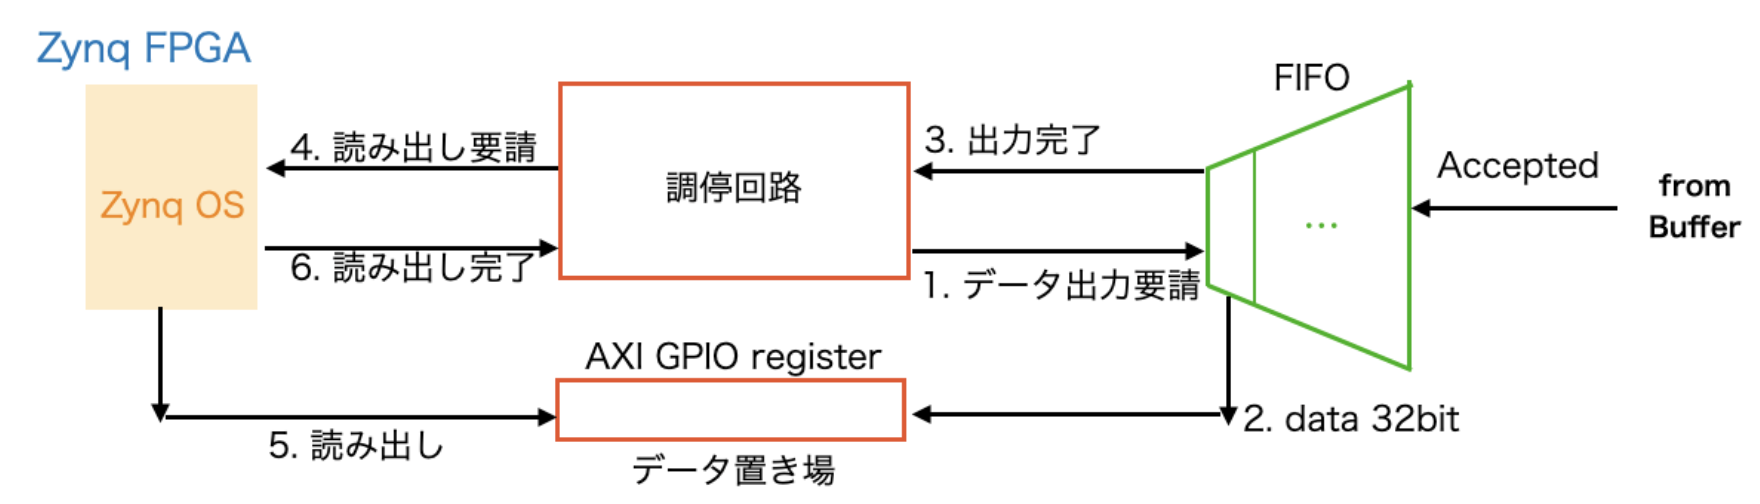
\includegraphics[width=16cm]{fig/QAQC/JATHubarbitator.png}
\caption[PLからPSでのデータ読み出しシステム概要]{PLからPSでのデータ読み出しシステム概要}
\label{JATHubarbitor}
\end{figure}

FPGAからUbuntuに読み出したいデータはFPGA内の動作クロックに乗せられFIFOメモリーにダンプされる。UbuntuからFIFOメモリーに直接アクセスする方法はないため、データのやり取りには工夫が必要となる。本システムではAXI GPIOレジスタを利用する。
AXI GPIOレジスタにはFPGAからもUbuntuからも任意のタイミングでアクセスすることができる。そのためUbuntuがデータを読み出す前にFIFOがデータを書き換えると、そのデータはUbuntuから読み出されずロスすることになる。またFIFOがデータを書き換える前にUbuntuが2回読み出し動作を行うと、同じデータが重複して読み出される。すべてのデータを漏れや重複なく読み出すために、FIFOとUbuntuのタイミングを取り持つ調停回路を作成した。調停回路は1 bitのフラグとステートマシンからなる。フラグはUbuntuとFIFO間の状況伝達に利用しており、0をFIFOからの書き込み待ち、1をUbuntuからの読み出し待ちと定義する。調停回路で実現される読み出しシークエンスを図\ref{JATHubarbitation}で示す。
\begin{figure} 
\centering
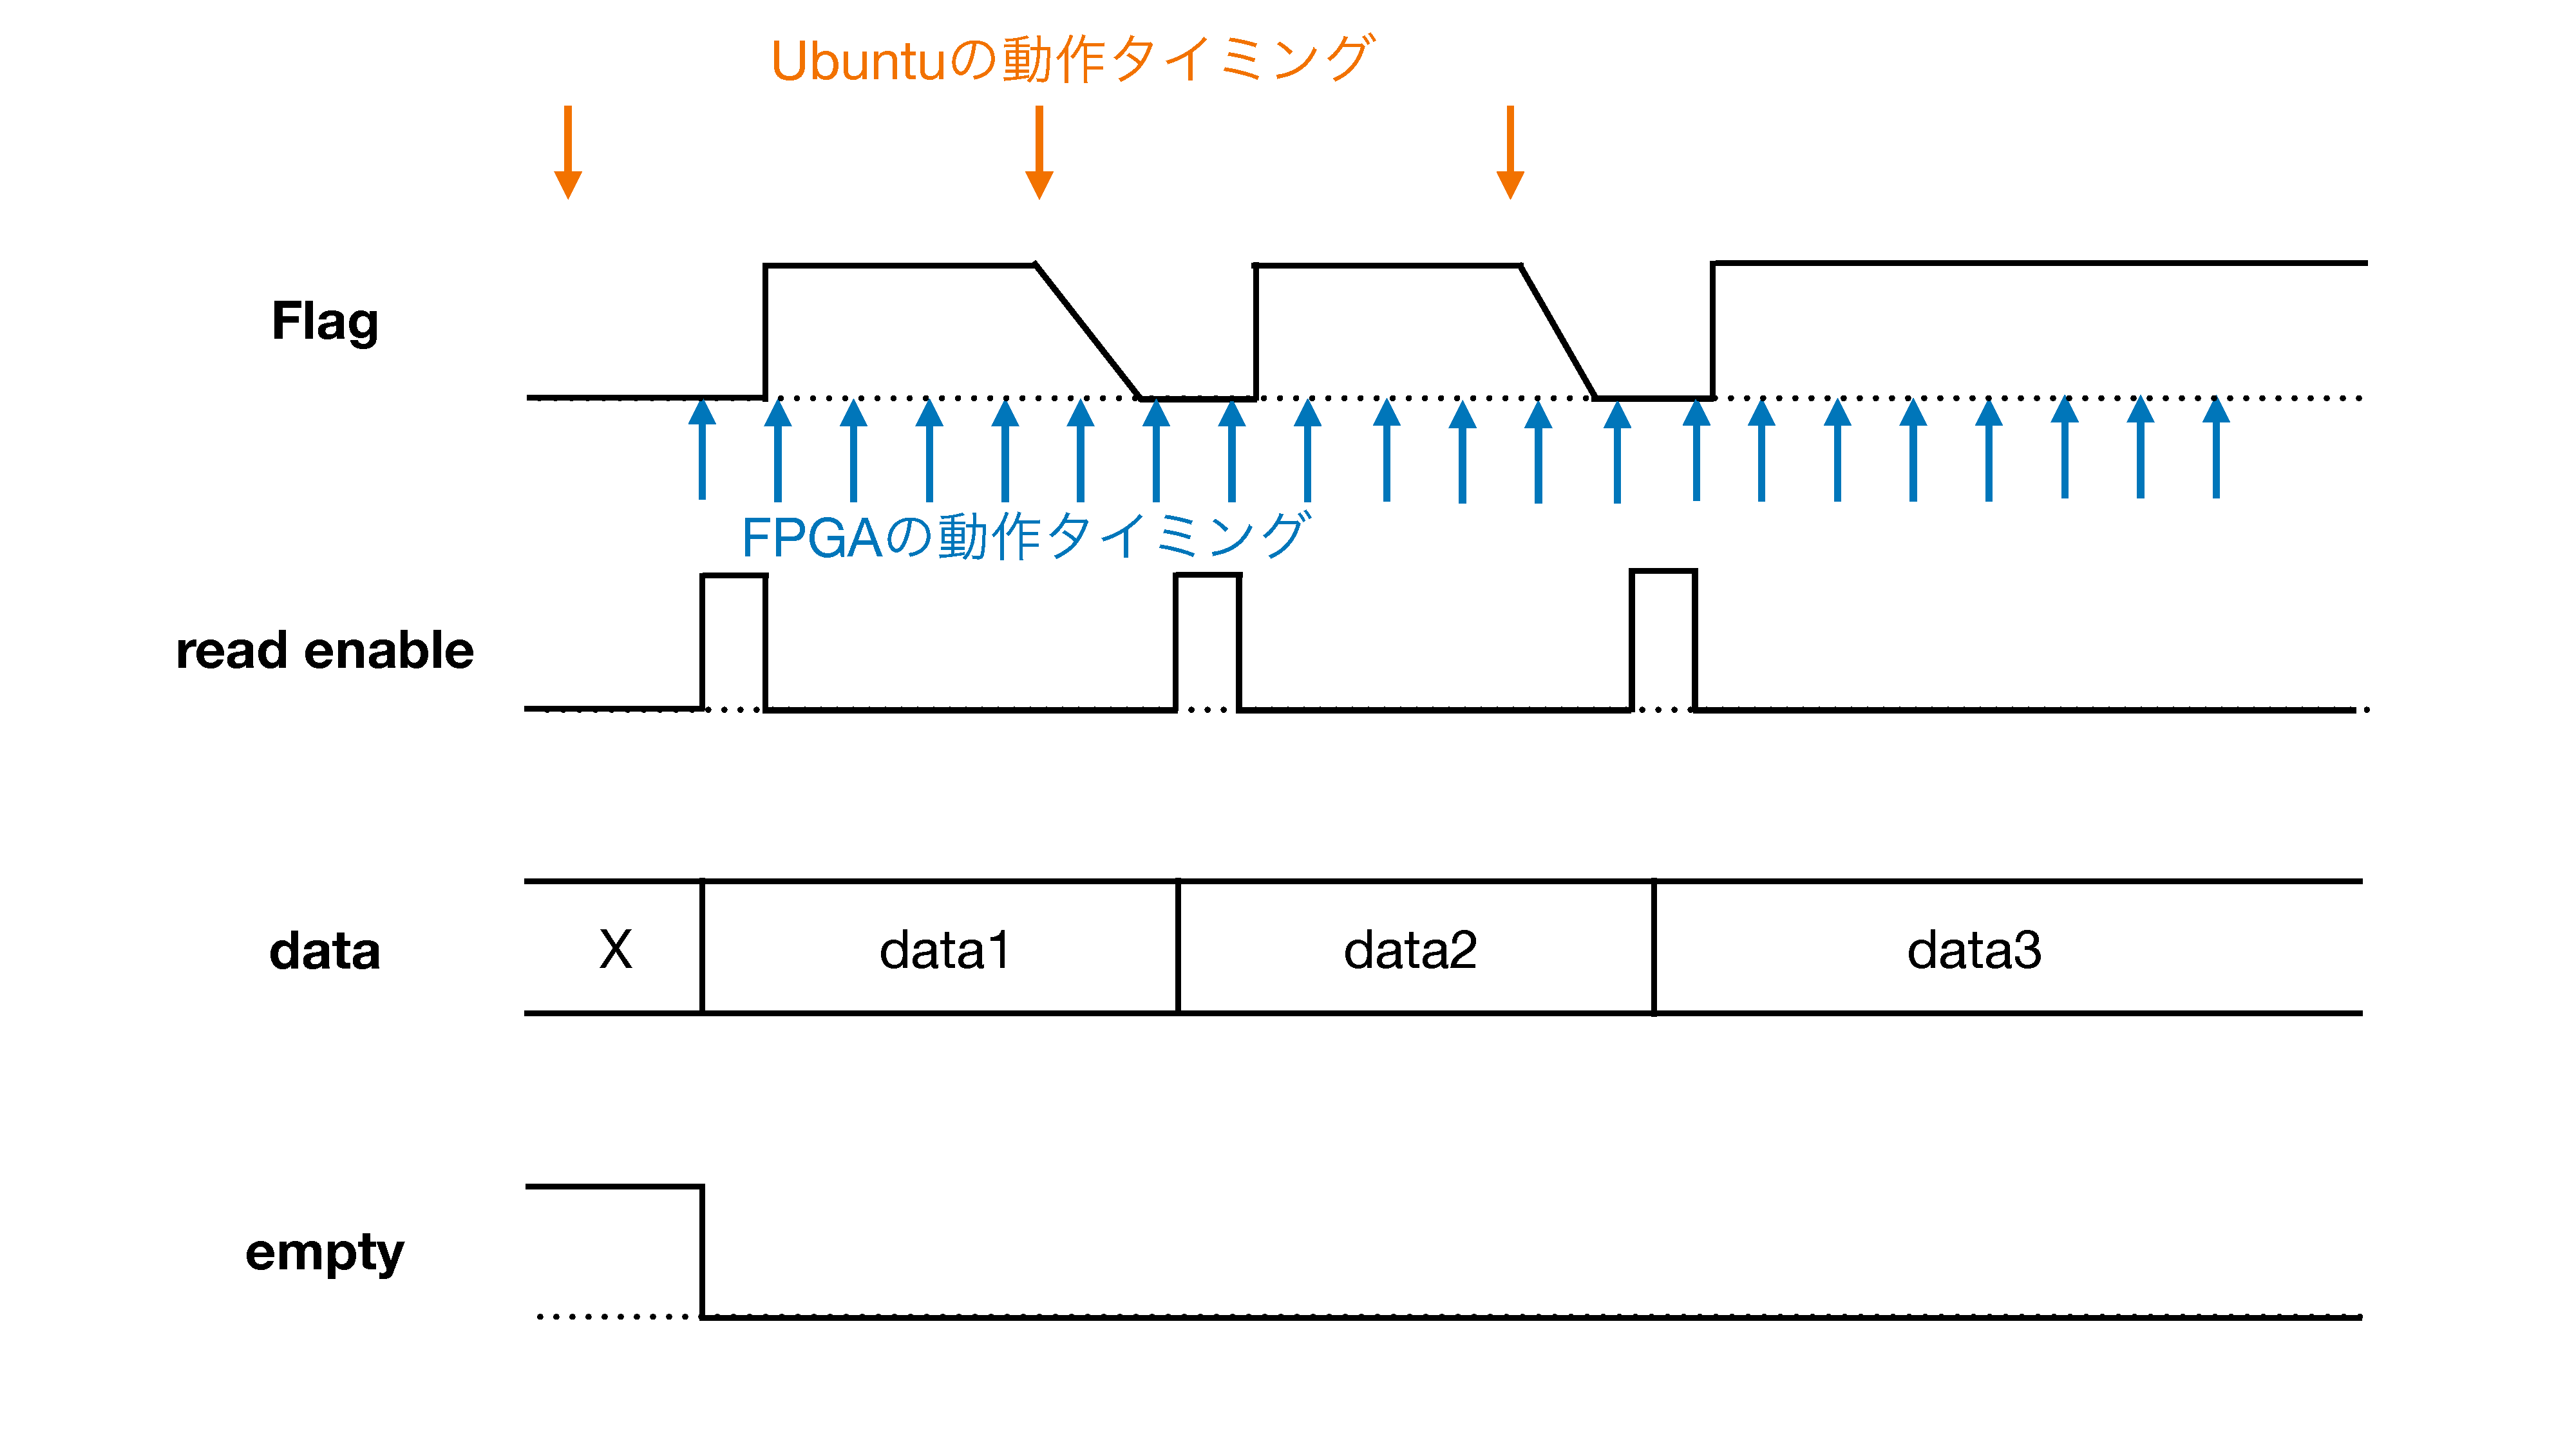
\includegraphics[width=16cm]{fig/QAQC/JATHubarbitation.png}
\caption[調停回路のシークエンス]{調停回路のシークエンス}
\label{JATHubarbitation}
\end{figure}

Ubuntu上のアプリケーションではフラグをモニターし、1になっていたらAXI GPIOレジスタの値を読み出し、その後フラグを1から0にさげる。FPGA上のステートマシンも同様にフラグをモニターし、0になったらFIFOにread enable信号を送信し、その後フラグを0から1に上げる。これによりAXI GPIO レジスタのデータ更新→データ読み出し→データ更新→データ読み出し…の順序が必ず保たれ、もれや重複のない読み出しが実現される。
作成した読み出しシステムの動作検証や性能評価は\ref{sec_PSboardQAQCdemo}節で行う。またこの読み出しシステムはPLからPSへの読み出しに複数箇所使われているため、以降汎用読み出しシステムと呼ぶ。


\subsection{FPGAの機能実装}
\label{subsec_function}
本節では\ref{sec_QAQCdesign}節で考案した試験を実行するために、QAQC用JATHub FPGAに実装した機能について述べる。
要請される機能はSLの働きをエミュレートする、PS board制御機能、ヒットデータ読み出し機能、JATHubの働きをエミュレートするJTAG/Recovery/Clock monitor機能である。
それ加え、JATHub1台でDAQを完結させるためにJATHub内部でTTC信号をエミュレートする機能、ファームウェア全体を制御するコントロール機能を実装した。
PS boardに送信するコントロール信号に関係する機能は200 MHzのTXユーザークロックを動作クロックとして利用する。PS boardから受信するデータを処理するパスでは200 MHzのRXユーザークロックを動作クロックに利用する。
開発を進めた2022年時点において、JATHubのファームウェアは完成していたためJTAG/Recovery/Clock monitor機能はそれをそのまま利用する。SLのファームウェアは開発が行われていなかったため、Run3で使われているSLのファームウェアを参考に開発を進めた。以下に各機能の詳細を説明する。

\subsection*{\textbf{コントロール機能}}
\label{subsubsec_control}
コントロール機能はQAQC用JATHubのファームウェア全体を制御するための機能であり、LHCバンチ交差クロックと同期する必要のないスローな制御を担当する。FPGA内のレジスタを制御し、読み出し機能やTTCエミュレート機能に使われる各パラメーターの変更をしたり、PS boardに送るコントロール信号を操作したりする。

\subsubsection{FPGA制御機能}
QAQC用JATHub上の各機能の制御はControl Centerから一元的に行う。
Control Centerでは複数のレジスタがインスタンス化されており、このレジスタを書き換えることでFPGA内の各機能を制御する。
レジスタのリストは付録\ref{}に添付する。Control Centerの操作はUbuntu上で実行したアプリケーションを起点に行う。
図\ref{JATHubccenter}にUbuntuとControl Centerの接続を示す。

\begin{figure} 
\centering
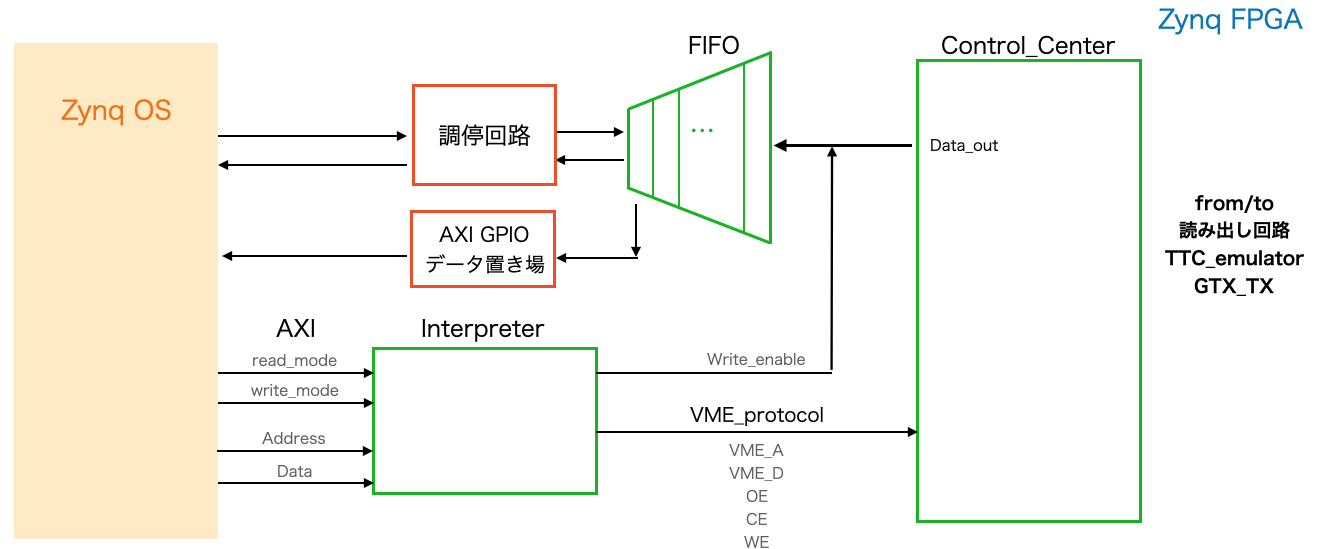
\includegraphics[width=16cm]{fig/QAQC/JATHubccenter.png}
\caption[JATHubコントロール回路]{JATHubコントロール回路。ZynqのOSからPL領域のControl Center内のレジスタを操作することによりFPGA内の各機能の制御やPS boardへのコントロール信号を制御する。OSからControl Center内のレジスタ操作はInterpreterが仲介する。ユーザーはアドレスとデータを指定することでVMEプロトコルに従ってレジスタの書き込みを行うことができる。データの読み出しには自作調停回路を利用しており、複数回の読み出しでも安全な設計が実現されている。}
\label{JATHubccenter}
\end{figure}

UbuntuからControl Center内のレジスタ操作は、VMEプロトコルを模倣した独自のプロトコルに従い、Interpreterがその操作を仲介する。ユーザーは、PSからアクセスしたいレジスタのアドレスと書き込みたいデータをInterpreterへ伝えることで、Interpreterがプロトコルに従ったバス操作を行い目的の動作を代行する。この実装によりPSからControl Center内のレジスタへ直接AXIバスを接続する必要がなく、PSからPLに伸びるAXIバスの本数を必要最小限にとどめることができる。また、PS領域とPL領域をつなぐバスが一つしかないため、Control Center内の複数のレジスタが同時に書き換えられることを防ぐ安全な設計になっている。Control Center からのデータの読み出しには 前述の汎用読み出し回路を利用した。

\subsubsection{PS board制御機能}

PS boardの制御はSLとPS board間で定められた通信フォーマット(図\ref{TGC_PSBdownlink})に従って、高速光通信を介して行われる。
QAQC用JATHubにもこのフォーマットに従ったパケット交換を行う機能を実装することで、PS boardのコントロールおよびLHCクロックの分配を行う。200 MHzのTXユーザークロックで動作するステートマシンにより40 MHzおきに5ワードを送信する。この時、40 MHzのLHCバンチ交差クロックの立ち上がりと同期したタイミングでワード0を送るように設計することで、40 MHzクロックに対して相対的な位相関係が固定されるよう実装されている。PS boardへ送るソフトリセット信号やテストパルストリガー信号はControl Center内のレジスタ操作により制御する。PS board FPGA内のレジスタ操作はワード2、ワード3に定義された16 bitのAddress、Command、Dataを用いて制御する。Commandにより書き込み/読み出し動作を決め、AddressでPS board内のレジスタアドレスを指定し、書き込み動作の場合はDataに設定した値を書き込む。
PS board上のDACやPP ASICを制御する方法として\ref{subsec_QAQCdesign}節では自立型制御機構を利用するものを述べた。QAQC用JATHubからPS boardを制御する際も、ワード1で定義されたCS BitmapおよびSCLK、SDI線をビットバンギングすることで、QSPIフラッシュメモリーにパラメータを書き込む。PS board FPGAの状態や各素子のモニターには自立型監視機構を利用する。DACの設定値、ADCの測定値、FGPAの温度、xADCによる供給電圧値などのモニター値は図\ref{PSBdataformat}に示すフォーマットに従い、6bitのデータタイプと4bitのデータに分割してQAQC用JATHubに送信される。たとえば16 bitのADCの値は4bitずつ4tickに分割して送信される。QAQC用JATHubは図\ref{JATHubmonitor}に示すように、分割されたモニターデータを再構成し、Control Center内のレジスタに自動で分配する。これによりUbuntuから任意のタイミングでControl Centerにアクセスしても、常に最新のモニターデータを取得することができる。
\vskip0.5\baselineskip

\begin{figure} 
\centering
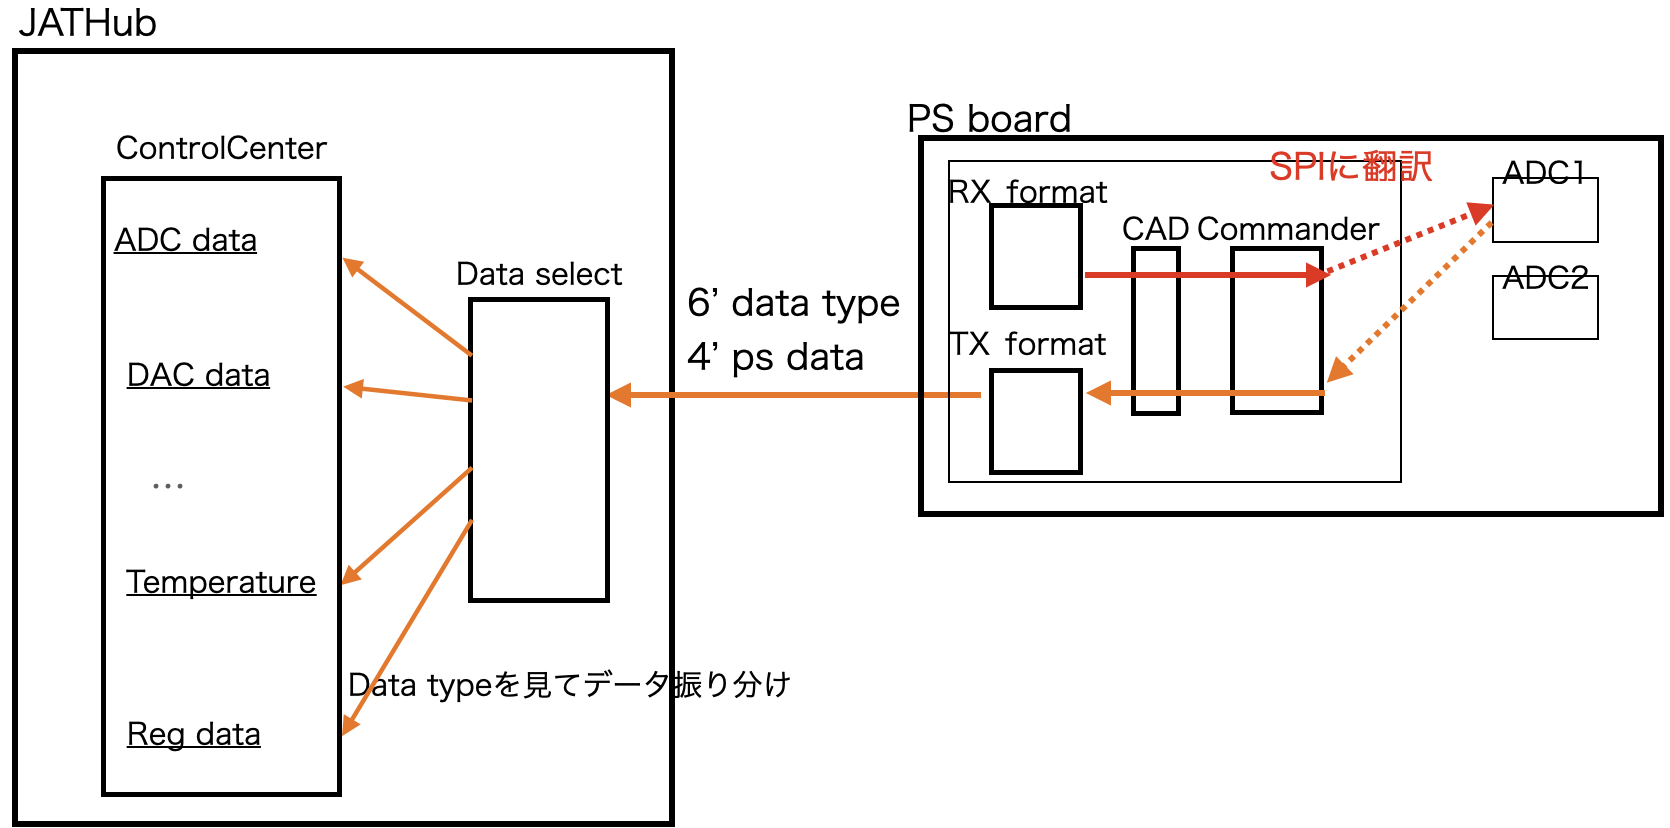
\includegraphics[width=16cm]{fig/QAQC/JATHubmonitor.png}
\caption[JATHub monitor]{JAThubに実装された監視機構。PS boardから送られる制御用データをデコードし、Control Center内のレジスタに格納する}
\label{JATHubmonitor}
\end{figure}

\begin{figure} 
\centering
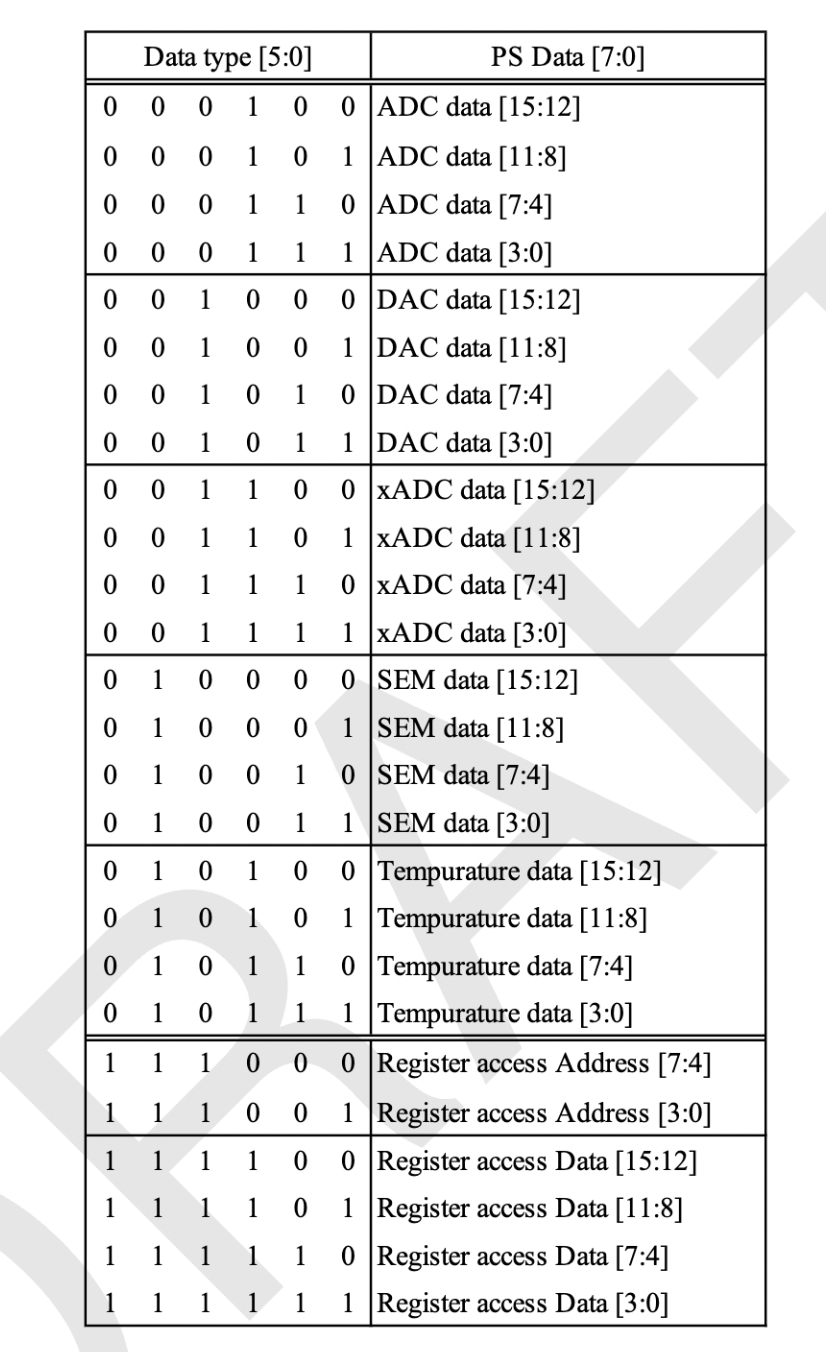
\includegraphics[width=10cm]{fig/QAQC/PSBdataformat.png}
\caption[PS boardから送信されるモニターデータのフォーマット]{PS boardから送信されるモニターデータのフォーマット}
\label{PSBdataformat}
\end{figure}

\subsection*{ヒットデータ読み出し機能}
\label{subsubsec_DAQ}
読み出し回路の役割はASDテストパルス試験において、PS boardから送信されるヒット信号をJATHub Zynq上のUbuntuから読み出すことである。JATHubは光通信を介してPS boardから25 nsごとに256 bitのヒット信号を受け取る。40 MHzで受け取るデータとそのデータに割り当てられたタイミング情報 (BCID、L1ID) をFPGA上でバッファーしておき (L1 Buffer)、TPTと同期してL1Aを発行することで、テストパルス信号に該当するタイミングのヒットデータを選択的に取り出すことができる。L1 BufferでAcceptされたデータはFIFOメモリーにダンプされ、ここからはCPUの動作する任意のタイミングでデータパスとは非同期で読み出される。
ヒットデータ読み出し機能の全体像を図\ref{JATHubdaq}に示す。
読み出し回路はTTC emulator、L1 Buffer、Derandomizer、Event Builderで構成される。DerandomizerのinputまではRXユーザークロックで動作しており、PS boardと固定位相で動作することが保証される。DerandomizerのoutputからはZynqのシステムクロックで動作しており、PSからFPGAにアクセスするAXIプロトコルと同じクロックドメインに属する。DerandomizerはFIFOで構成されていて、inputとoutputを非同期に動作させることができる。以下に各モジュールの役割を説明する。

\begin{figure} 
\centering
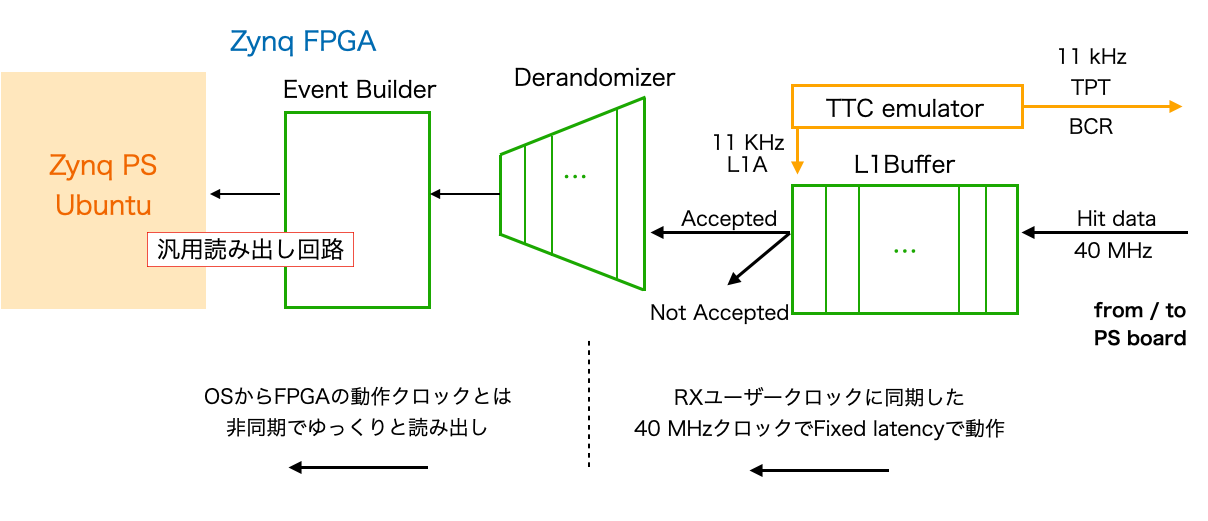
\includegraphics[width=16cm]{fig/QAQC/JATHubdaq.png}
\caption[読み出し回路の全体像]{読み出し回路の全体像}
\label{JATHubdaq}
\end{figure}

\subsubsection{TTC emulator} \par
ASDテストパルス試験ではJATHub、PS board、ASDの間で固定位相でLHCバンチ交差クロックを分配して、それぞれのエレクトロニクスが同期して動作する必要がある。TGCシステムではLHCバンチ交差クロックはCTPから分配されるが、本試験システムではJATHub1台で試験を完結させるため、JATHub上の水晶発振器で生成されたクロックをLHCバンチ交差クロックとして扱う。具体的には水晶発振器をもとに作られた200 MHz TXユーザークロックを分周して40 MHzクロックを作る。Bunch Counter Reset (BCR) 信号やEvent Counter Reset (ECR) などのイベントビルディングに必要なTTC信号もJATHub内で生成しPS boardへと分配する。この役割を果たすのがTTC emulatorである。ここで発行されたTTC信号はコントロール信号のワード0に埋め込まれ、光ファイバーを介してPS boardへと伝えられる。L1A信号もTTC emulatorから出力され、前述したようにTPTとL1Aを同期して管理することでFixed latencyのDAQを実現している。以下にTTC emulatorのサブモジュールを説明する。
\vskip0.5\baselineskip

\begin{itemize}
    \item {TTC generator : } 40MHz LHCバンチ交差クロックで動作するカウンター。reset信号でカウンターをリセットし、1クロックチック毎にカウンターの値を1つずつインクリメントする。カウンターの値が3564に達したタイミングでBCR信号を発行する。デフォルトの設定ではTPT、L1AもBCRに合わせて3564 BCに一回発行しているが、TPT、L1Aの発行頻度は任意の値に設定することができる。TPT lengthを変更することで、TPTを複数BCに渡って出力することも可能になっている。
    \vskip0.5\baselineskip

    \item{TTC Delay : }1bit幅、深さ4096のBRAMで実装したdelay回路。L1A、BCR、TPTに任意の遅延をかけることができる。L1A Delayを調整することでTPTからL1Aを発行するまでのレイテンシーを変更することができる。
    \vskip0.5\baselineskip

    \item{ID counter : }BCR、ECR、L1Aを受けてBCID、ECID、L1IDを数え上げるカウンター。ここで発行されたBCIDやL1IDはUbuntuからの読み出しフォーマットに組み込まれて出力される。読み出したデータにおけるL1IDの連続性やBCIDを確認することでデータの欠損や重複をチェックすることができる。
    \vskip0.5\baselineskip
    
    \item{FPGAテストパルス発行機能 : }PS boardの持つFPGAテストパルスを発行するためのモジュール。FPGAテストパルスはPS board内のBRAMに保存される。BRAMのaddressを指定した状態で、TPTを発行するとBRAMから256 bitのヒットビットマップが取り出され、ASDからのヒット信号の代わりにJATHubに送信される。
    \vskip0.5\baselineskip
\end{itemize}

\subsubsection{L1 Buffer} \par
L1 BufferはPS boardから受信した256 bitのヒット信号とECRID、L1ID、BCIDなどのタイミング情報を合わせた432 bitのデータを一時的に保管するためのリングバッファーである。TTC emulatorからL1Aが出されたイベントは後段のDerandomizerに転送され、それ以外のデータはここで捨てられる。25 nsごとに到着するヒット信号は、書き込み用ポインタが指すアドレスに格納される。書き込み用ポインタと読み出し用ポインタはLHCバンチ交差クロックに同期して、1ずつインクリメントする。書き込み用ポインタがBRAMの最後尾まで達した場合、次のクロックチックで再び先頭に戻る。L1 depthによって書き込み用ポインタと読み出し用ポインタのアドレスの差を設定することができ、Bufferの深さを任意の値に設定できる。また、L1Aが発行されてから何BC分のデータを読み出すかをReadoutBCによって設定することができる。デフォルトでは3に設定されており、一回のL1Aに対してprevious、current、nextの3バンチ分のデータ読み出す。ReadoutBCで設定されたBC分のデータを読み出している途中に再度L1A信号を受信すると、読みだしエラーを出力する。読み出しエラーが生じた場合、そのL1IDをControl Center内のレジスタに格納しユーザーが確認できるようになっている。
\vskip0.5\baselineskip

\subsubsection{Derandomizer} \par
Derandomizerは、後段で行われる読み出しの処理待ちバッファーであり、432 bitの入力データを32 bitずつ出力する。DerandomizerはFIFOを2つ直列に並べることで実装している。
データの分割にはFIFO IPのスライス機能\footnote{FIFO IPでは入力bit幅の1/2、1/4、1/8のbit幅での出力が可能である。}を利用している。Derandomizerの出力はUbuntuのInt型と整合性のある32bitが好ましい。そこで432 bitの入力データに不要な64 bitのデータを加え、512 bitのデータを2つのFIFOで1/4ずつスライスすることで、最終的な出力を32 bitにしている。64 bitの不要データは1つ目のFIFOと2つ目のFIFOの間で捨てられ、Ubunutuからの読み出しには関係しない。\par
FIFOは入力されたデータを順番に出力する特性を持ったメモリーである。書き込みと読み出しを非同期に行うことができ、一般にクロックドメインをまたぐデータの送受信に利用される。本システムでは固定レイテンシーで動くFPGA内の読み出し回路とPS領域からのデータ読み出しをつなぐ目的で使用する。Derandomizerへの書き込み動作はRXユーザークロックと同期した40 MHzクロックを動作クロックに動作し、読み出しはUbuntuからゆっくりと行う。Derandomizerへのデータ書き込みレートがUbunruからの読み出しレートを上回る場合には、Derandomizerのoccupancyは増大していく。その状態が続くとバッファーのオーバーフローが発生し、データが欠損する。バッファーオバーフローが生じた場合の対応は後に紹介する。
\vskip0.5\baselineskip

\subsubsection{Event Builder} \par
Event BuilderはDeradomizerに格納された32bit幅のデータを240 MHzのクロックチック毎に1ワードずつ順番に読み出し、イベントごとにパッケージする。図\ref{JATHubhitformat}に1イベント分の読み出しフォーマットを示す。PS boardから受信した256 bit $\times$ 3 BC分のデータに加えて、TTC emulator から発行されたTTC信号 (ECRID、L1ID、BCID)、PSBで発行されたBCIDも同時に読み出す。JATHub内で割り当てられたBCIDとPS boardから返ってきたBCIDの差を確認することで、固定レイテンシーでのデータ読み出しが実現されているか確かめることができる。
\vskip0.5\baselineskip

\begin{figure} 
\centering
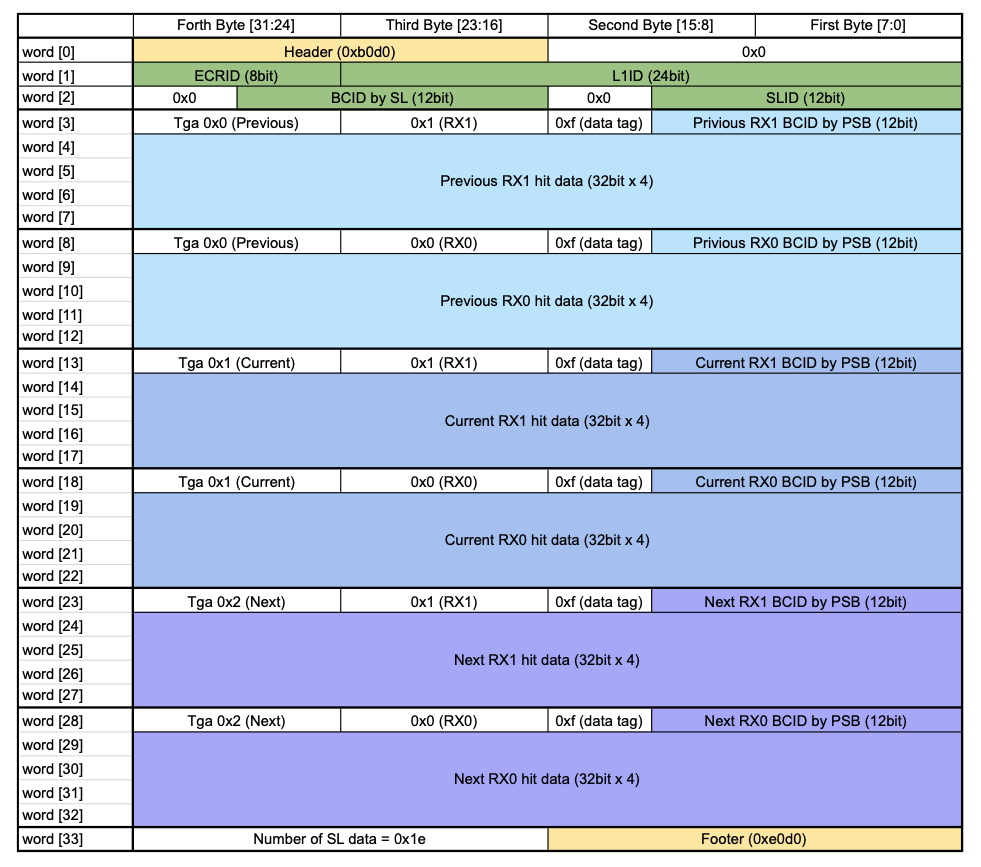
\includegraphics[width=16cm]{fig/QAQC/JATHubhitformat.png}
\caption[JATHubからのヒットデータ読み出しフォーマット]{JATHubからのヒットデータ読み出しフォーマット}
\label{JATHubhitformat}
\end{figure}

\subsubsection{読み出し回路の性能} \par
実装した読み出し回路における、読み出しレートの上限を概算することは、QAQC試験を設計するにあたり重要である。ASDテストパルス試験におけるTPT発行レートはこれにより決められる。Ubuntu上でDerandomizerからデータを読み出し続けるアプリケーションを走らせ、FIFOに格納された1000イベント分のパケットを読み出すのにかかる時間を測定した。
図\ref{JTAHubreadspeed}にその結果を示す。横軸に読み出したパケット数、縦軸に経過時間(s)をとる。得られた測定結果を線形フィットし、その傾きから1パケット読み出すのにかかる時間を概算した。その結果、1イベント分のデータを読み出すのにおおむね$85\,\mu\mathrm{s}$かかることがわかった。

\vskip0.5\baselineskip
\begin{figure} 
\centering
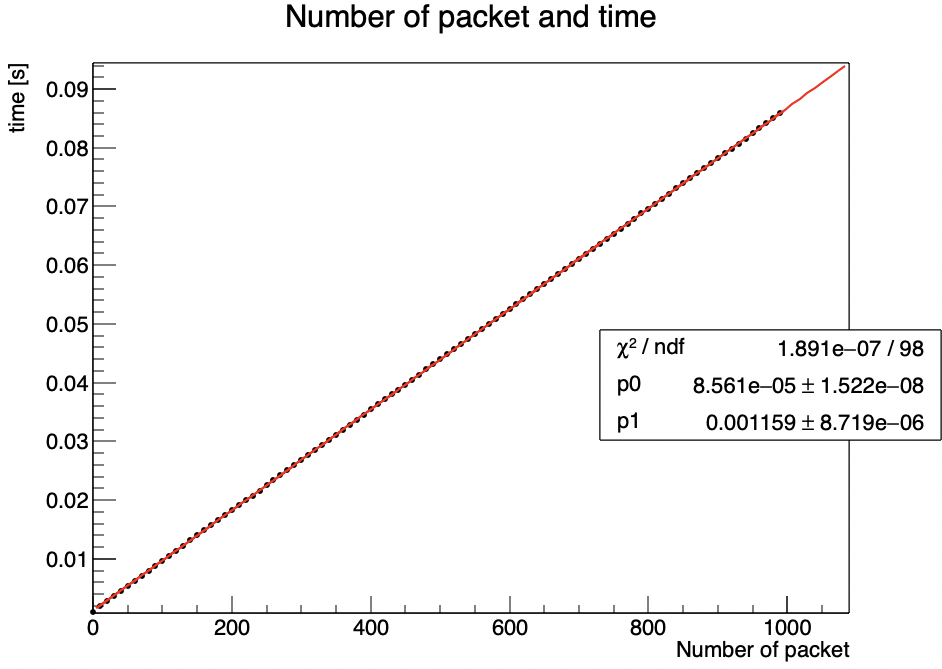
\includegraphics[width=16cm]{fig/QAQC/JTAHubreadspeed.png}
\caption[PSからのヒットデータ読み出し速度の測定]{PSからのヒットデータ読み出し速度の測定}
\label{JTAHubreadspeed}
\end{figure}

\subsubsection{バッファーオーバーフローへの対応} \par
万が一バッファーオーバーフローが生じた時においてもイベントパケットが崩れることのないよう、Derandomizerにはバックプレッシャー機能を実装した。Derandomizerのoccupancyがあらかじめ設定した容量閾値 (4000/4096) を超えると、L1 Bufferへalmost full信号が送られる。almost full信号を受け取ったL1 Bufferは、処理中のイベントのデータ出力を完遂させたのち (previousの出力中にalmost full信号が来た場合、current、nextのデータまで出力を終えた後) 、データの出力を一時的に停止する。Ubuntuからのデータ読み出しが進み、Derandomizerのoccupancyが容量閾値を下回ると、再びデータの出力を再開する。これにより、任意のタイミングで読み出しを開始/終了してもイベントのパケットを崩すことなくデータを読み出すことができる。
ASDテストパルス試験ではUbuntuから読み出したイベント数を分母に、ヒットデータが入っていた割合をefficiencyとして定義する。そのため、この実装により、読み出し回路にバッファーオーバーフローが生じた場合でもefficiencyを正確に測定することができる。
\vskip0.5\baselineskip

\begin{figure} 
\centering
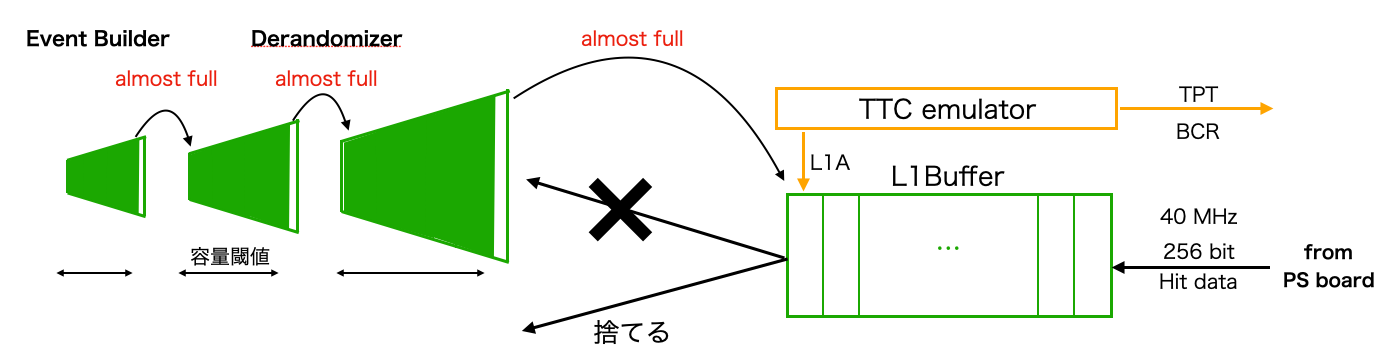
\includegraphics[width=16cm]{fig/QAQC/JATHubbackpressure.png}
\caption[リードアウト回路におけるバックプレッシャー機能]{リードアウト回路におけるバックプレッシャー機能}
\label{JATHubbackpressure}
\end{figure}

\section{PS board QAQC試験デモンストレーション}
\label{sec_PSboardQAQCdemo}

\subsection{試験環境}
\label{subsec_testenv}
東京大学に設置したテストベンチを利用して、開発したQAQC用JATHubの動作検証およびQAQC試験のデモンストレーションを行なった。
セットアップを図\ref{QAQCsetup}に示す。QAQC用のJATHubはVMEクレートに設置しバックプレーンのJ3コネクターを通じて給電する。PS boardには3.3 Vデジタル電源、3.0 V、-3.0 Vアナログ電源を用意しデスクトップで給電する。QAQC用JATHubとPS boardは3本の光ファーバーと2本のCat-6ケーブルで接続する。1台のPS boardには8台のASDをシグナルケーブルで接続する。

\begin{itembox}{図QAQCsetup}
    3号館のセットアップの良い写真を撮ってくる
\end{itembox}

\vskip\baselineskip

\subsection{デモンストレーションの結果}
\label{subsec_tb_result}
QAQC試験では量産個体に対する試験に先んじて、PP ASICの遅延、DACの閾値電圧、L1A depthなどセットアップに依存する制御パラメーターを設定しておく必要がある\footnote{ここで決めるパラメーターはQAQC試験を行うためのパラメーターであり、実験時には改めてパラメーターを決めるための調査が行われる。}。
以下に各パラメーターを定めるために行った事前試験の内容とその結果を示す。

\subsubsection{PP ASIC遅延パラメーター}
PP ASICの遅延パラメーターは使用するシグナルケーブルの長さに依存するパラメーターである。ASDからのテストパルス信号の立ち上がりがPP ASIC陽子バンチ識別回路におけるLHCバンチ交差クロックの立ち上がりと極めて近い場合、イベントごとにアサインされるBCIDが1つに定まらない可能性がある。これを防ぐため、PP ASICの可変遅延回路の遅延パラメーターを変更し、両者の立ち上がりが十分離れるよう調整する。このパラメーターの決定のためディレイスキャンを行なった。ディレイスキャンとは、PP ASICの遅延パラメーターを1stepずつ変更しながらデータを取得し、アサインされたBCIDの変化をみるものである。結果を図\ref{QAQCdelayscan}に示す。横軸に設定した遅延の大きさ、縦軸にefficiencyを表す。この測定では陽子バンチ識別回路の有効ゲート幅を25 ns、可変遅延回路の刻み幅を1.19 nsに設定している。遅延パラメーターを変更していくと、陽子バンチ識別回路でアサインされるBCがprevious → current → nextと遷移していく様子がわかる。current BCのプラトー領域にヒットが返ってくるよう、QAQC試験で利用する遅延パラメーターは20 nsと決定した。
\vskip0.5\baselineskip

\begin{figure} 
\centering
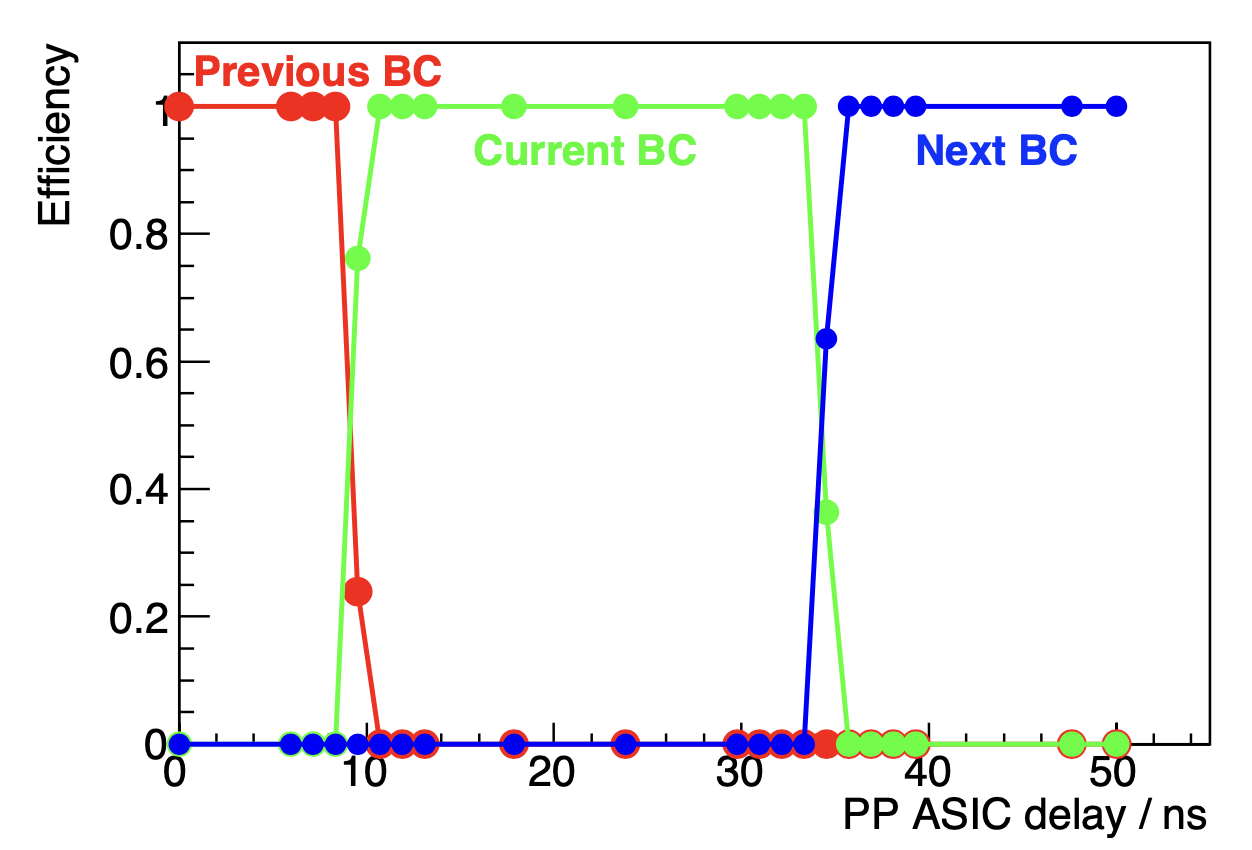
\includegraphics[width=16cm]{fig/QAQC/QAQCdelayscan.png}
\caption[ディレイカーブ]{テストベンチで測定したdelay curve}
\begin{itembox}{要更新}
    これは青木さんの結果。自分で取り直したものに差し替える。
\end{itembox}
\label{QAQCdelayscan}
\end{figure}

\subsubsection{L1Adepth}
L1A depthはL1 Bufferの深さを決めるパラメーターであり、TTC emulatorでTPTを発行してからPS board からヒットデータが返ってくるまでのレイテンシーに合わせて調整する必要がある。主にPS boardからJATHubの間の光ケーブルの長さに依存するパラメーターである。このパラメーターはディレイスキャンと同時に設定を行なっており、0x85に設定した。
\vskip0.5\baselineskip

\subsubsection{ノイズスキャン}
DACの閾値電圧は使用するASDのノイズの大きさに依存して変えるべきパラメーターである。ASDをには$\mathcal{O}(10 \,\mathrm{mV})$のノイズが乗っていることが知られており、それよりも閾値電圧を低く設定してしまうと、ノイズをヒット信号として処理してしまう。閾値電圧はノイズの値よりも高く、かつテストパルスの波高より十分低く設定すべきである。そこで、DACの閾値電圧を変えながらテストパルスを測定するノイズスキャンを行なった。その結果を図\ref{QAQCnoisescan}に示す。
1台のPS boardに搭載される16台のASDに印加する閾値電圧をコヒーレントに変えていき、ヒットのefficiencyを測定した。閾値電圧が0 mV程度になるとノイズによるヒットが見られるようになってきて、50 mV以上の閾値電圧をかけるとノイズが消えていく。この結果から本セットアップでのDAC閾値は+-それぞれ+70 mV、-40 mVと設定した。
\vskip0.5\baselineskip

\begin{figure} 
\centering
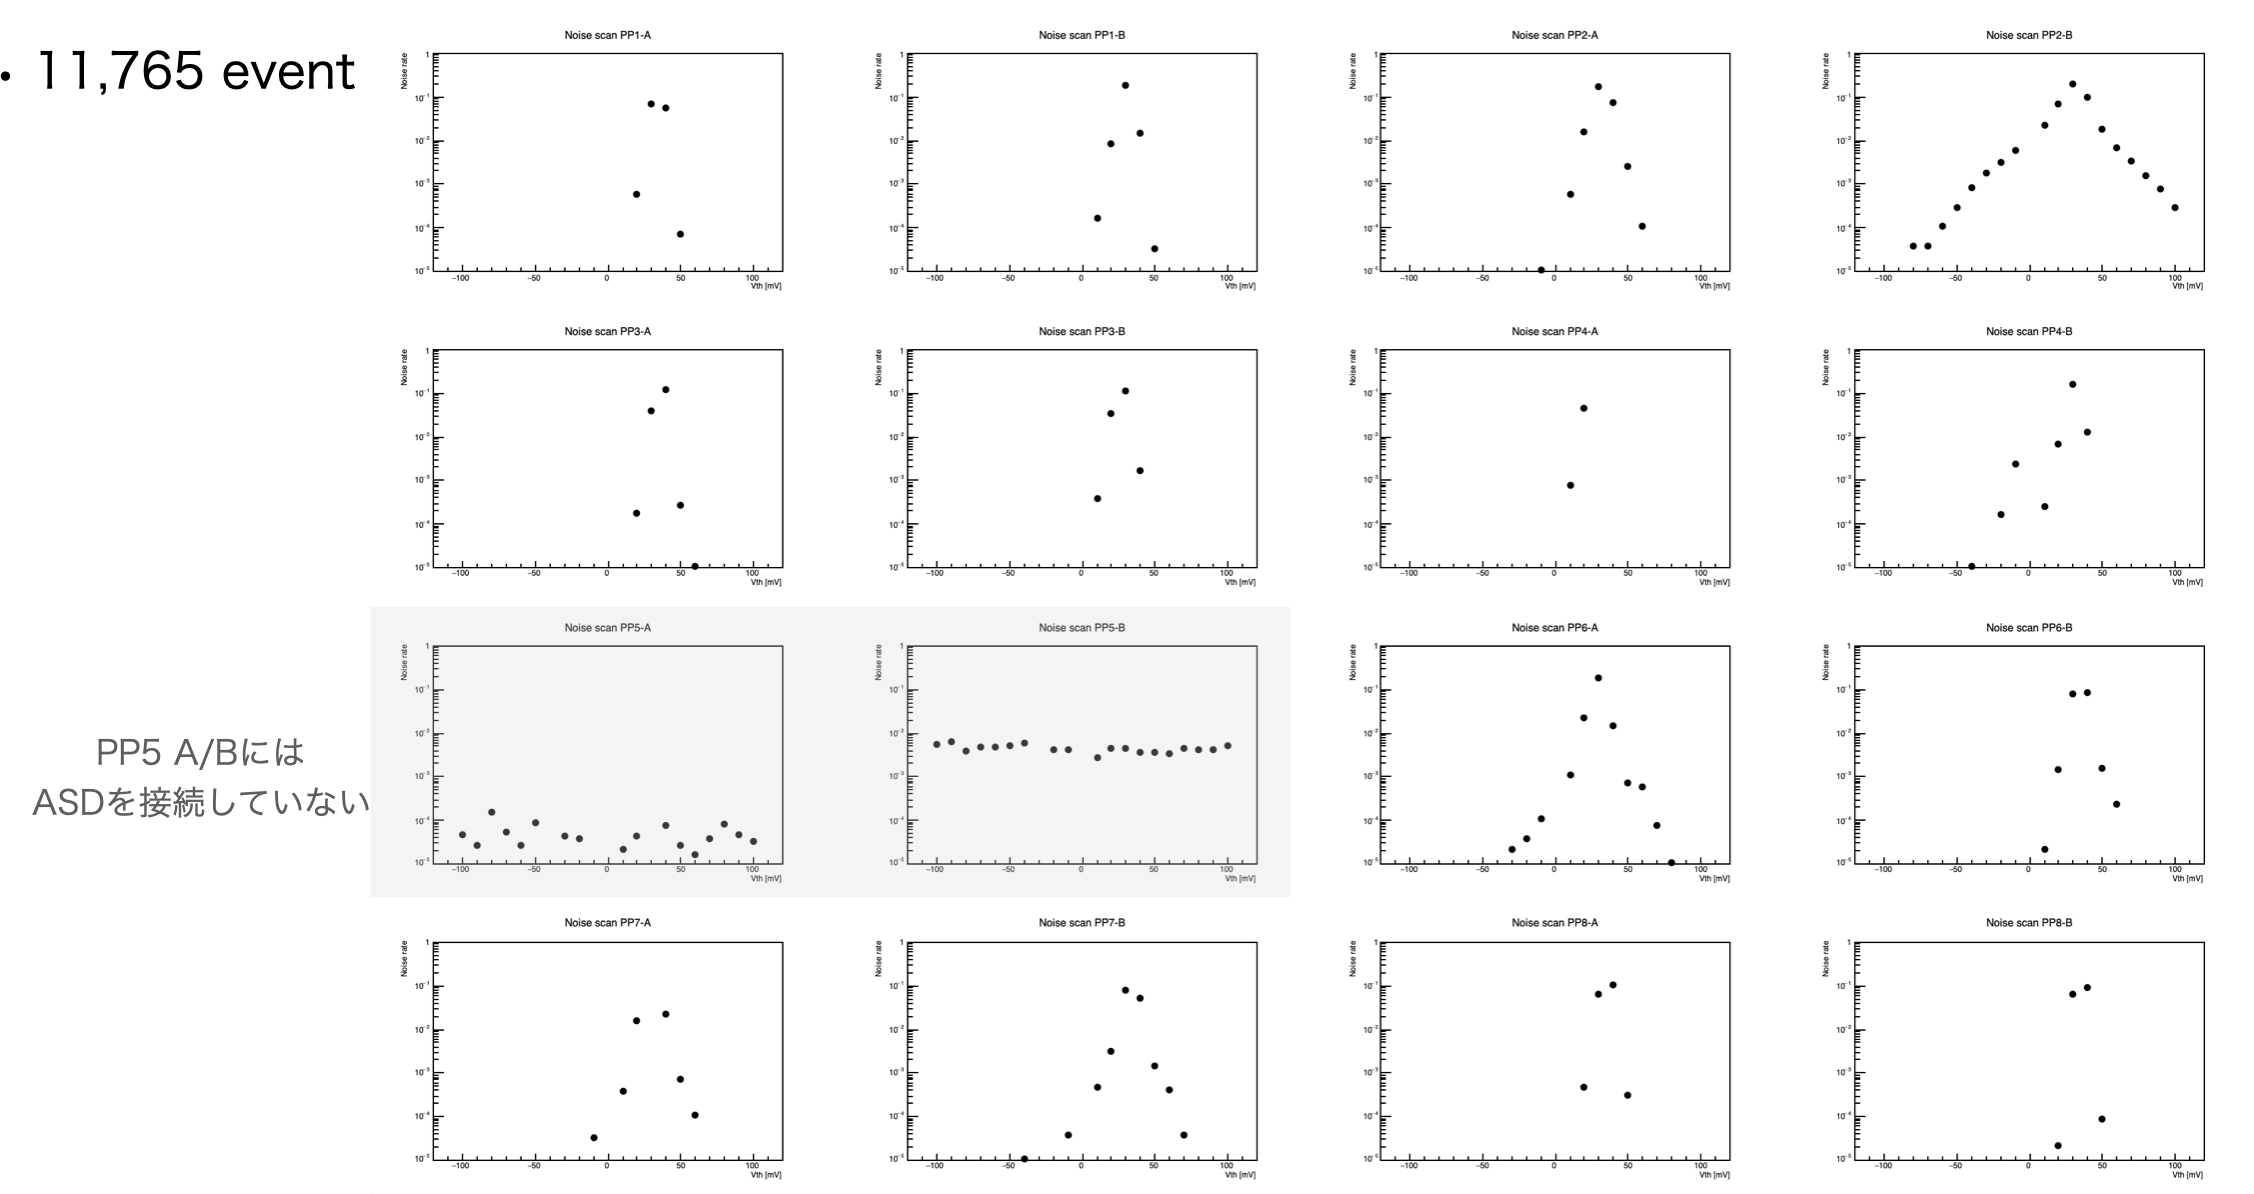
\includegraphics[width=16cm]{fig/QAQC/QAQCnoisescan.png}
\caption[ノイズスキャン]{ノイズスキャンの結果}
\begin{itembox}{要更新}
    3号館でとりなおす。16台の結果を重ね書きしたものに更新。
\end{itembox}
\label{QAQCnoisescan}
\end{figure}

これらのパラメーターをもとにASDテストパルス試験を行なった結果を図\ref{QAQCresult}示す。この試験ではパラメーターは固定した状態で10,000回TPTを発行した時の、Previous、Current、Nextそれぞれのefficiencyを測定している。結果はすべてのチャンネルでCurrentのefficiencyのみが1となっており、PS board上の各種パラメーターの設定が期待通り行えていること、また固定レイテンシーでの読み出しが実現できていることを確認することができた。

\begin{figure} 
\centering
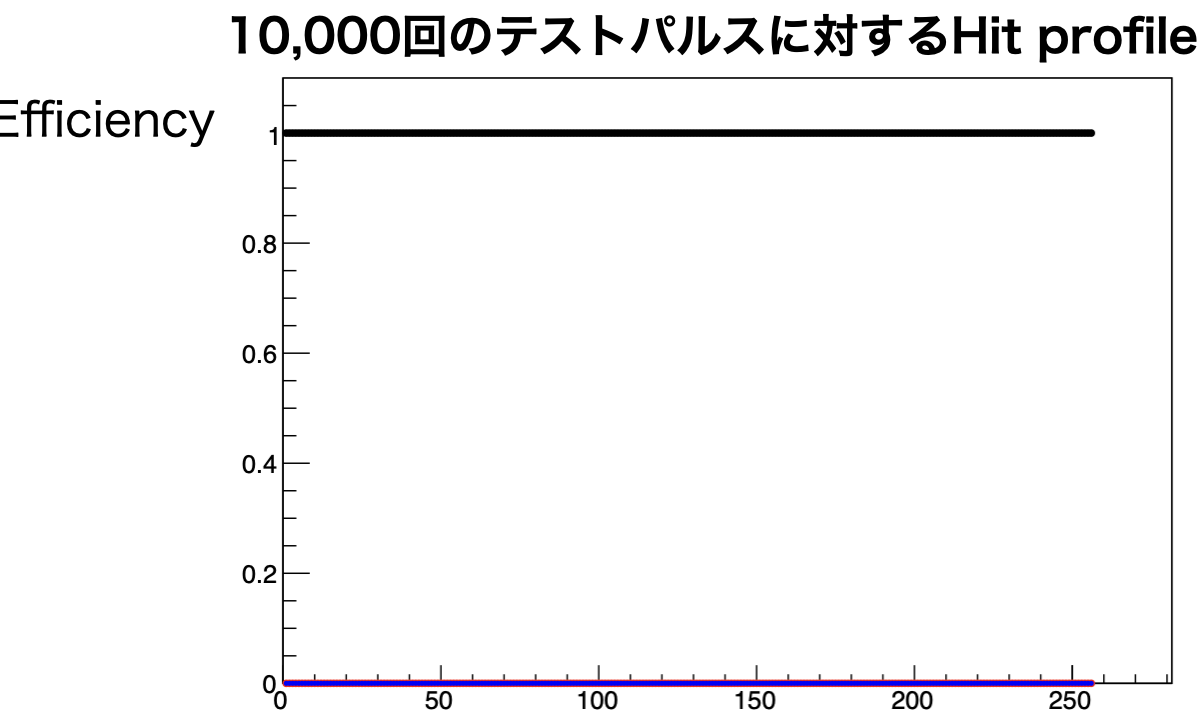
\includegraphics[width=16cm]{fig/QAQC/QAQCresult.png}
\caption[ASDテストパルスの結果]{ASDテストパルス試験の結果}
\label{QAQCresult}
\end{figure}

その他の試験においても期待通りの結果が得られ、QAQC用JATHubシステムの実装がうまくいっていることを確認することができた。表\ref{table_testtime}各試験の所要時間を示す。

\begin{table}[]
    \centering
    \caption{各試験にかかる所要時間}
    \label{table_testtime}    
    \begin{tabular}{ll}
    \hline
    試験項目                          & 所要時間   \\ \hline
    SVFプレイヤーによるQSPIファームウェア書き込み    & 40 min \\
    QSPIパラメーター書き込みおよび読み出し         & 2 min  \\
    リカバリー試験                       & 1 s    \\
    電圧値のモニタリング (ADC、xADC) & 2 s    \\
    Clock位相測定                     & 30 s   \\
    ASDテストパルス試験                   & 10 s  
    \end{tabular}
\end{table}

\subsection{試験並列化のためのシステムアップグレード}
\label{subsec_parallel}
QAQC試験のデモンストレーションにより、1枚のPS boardを試験するのに配線作業等も含めると、合計50分以上時間かかることが明らかになった。1500枚のPS boardに対して試験を行うには、24時間試験をやり続けたとしても2ヶ月程度かかる見込みで、現実的なタイムスケールで試験を完了させるためには試験の高速化が求められる。単純にはQAQC用JATHub1台とPS board1台のセットアップを複数用意することが考えらるが、QAQC用JATHubに必要なイーサーネット通信のためのRJコネクターと光通信のためのSFP+コネクターを両方有しているものは、世界に1台しか存在しない(JATHub 試作1号機)。並列化のためには新たなシステム設計が必要となる。そこで考案された並列化システムのセットアップを図\ref{QAQCpararell}に示す。システムのコンセプトは、試作1号機をQAQCマスターとして利用し、QAQCマスターから20台のQAQC用JATHub\footnote{RJコネクターをもたないJATHub量産機} (QAQCスレーブ) を操作することである。ユーザーはQAQCマスターのみを操作して、QAQCスレーブに対して試験開始を命令したり、試験状況を監視したりする。QAQCマスターとQAQCスレーブの通信を中継する目的でTAMボードも利用する。QAQC用マスターとTAMの通信は光ファイバーを介したシリアル通信を用い、TAMとQAQCスレーブの通信はバックプレーンを通じたVME通信を用いる。
\begin{figure} 
    \centering
    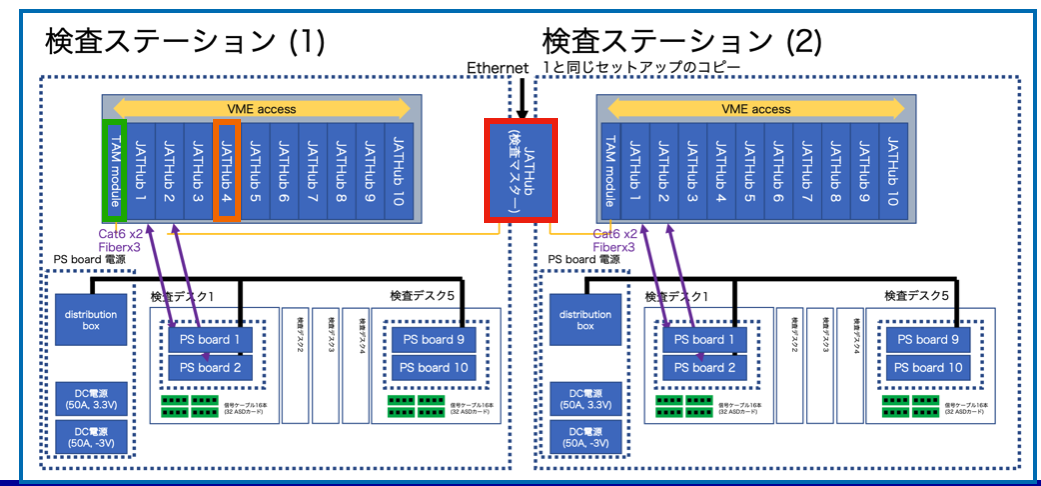
\includegraphics[width=16cm]{fig/QAQC/QAQCpararell.png}
    \caption[並列化システムの概要]{並列化システムの概要}
    \label{QAQCpararell}
\end{figure}

QAQCスレーブのUbuntuは起動と同時に試験用アプリケーションを走らせ、マスターから試験開始を伝えるためのレジスタをポーリングする。マスターから合図が届くと自動で、1台のPS boardに対する試験を遂行し始める。各試験の結果は2 bitのstatus bitで表され\footnote{0をidle、1をsuccess、2をfailで定義する}、QAQCマスターは任意のタイミングでそれを確認することができる。開発したアプリケーションによる試験ステータスモニターの例を図\ref{QAQC_monitor}に示す。またQAQCスレーブは各試験の詳細なログをとっておき、ローカルのSDカード上に保存する。もし試験で問題が発覚した個体が発生した場合は、このログを見ることで問題を詳細に把握することができる。
並列化システムについても、東京大学でテストベンチを構築し動作検証を行なった。図\ref{QAQCpararellpicture}にセットアップを示す。QAQCマスター、TAM、QAQC用スレーブ1台、PS board1台、ASD 8台を用いたミニマムなセットアップになっている。QAQCマスターの試験開始から、試験の終了まで問題なく動作することができ、2024年から始まる1500枚の試験に向けて準備が整えられていることを確認した。

\begin{figure} 
\centering
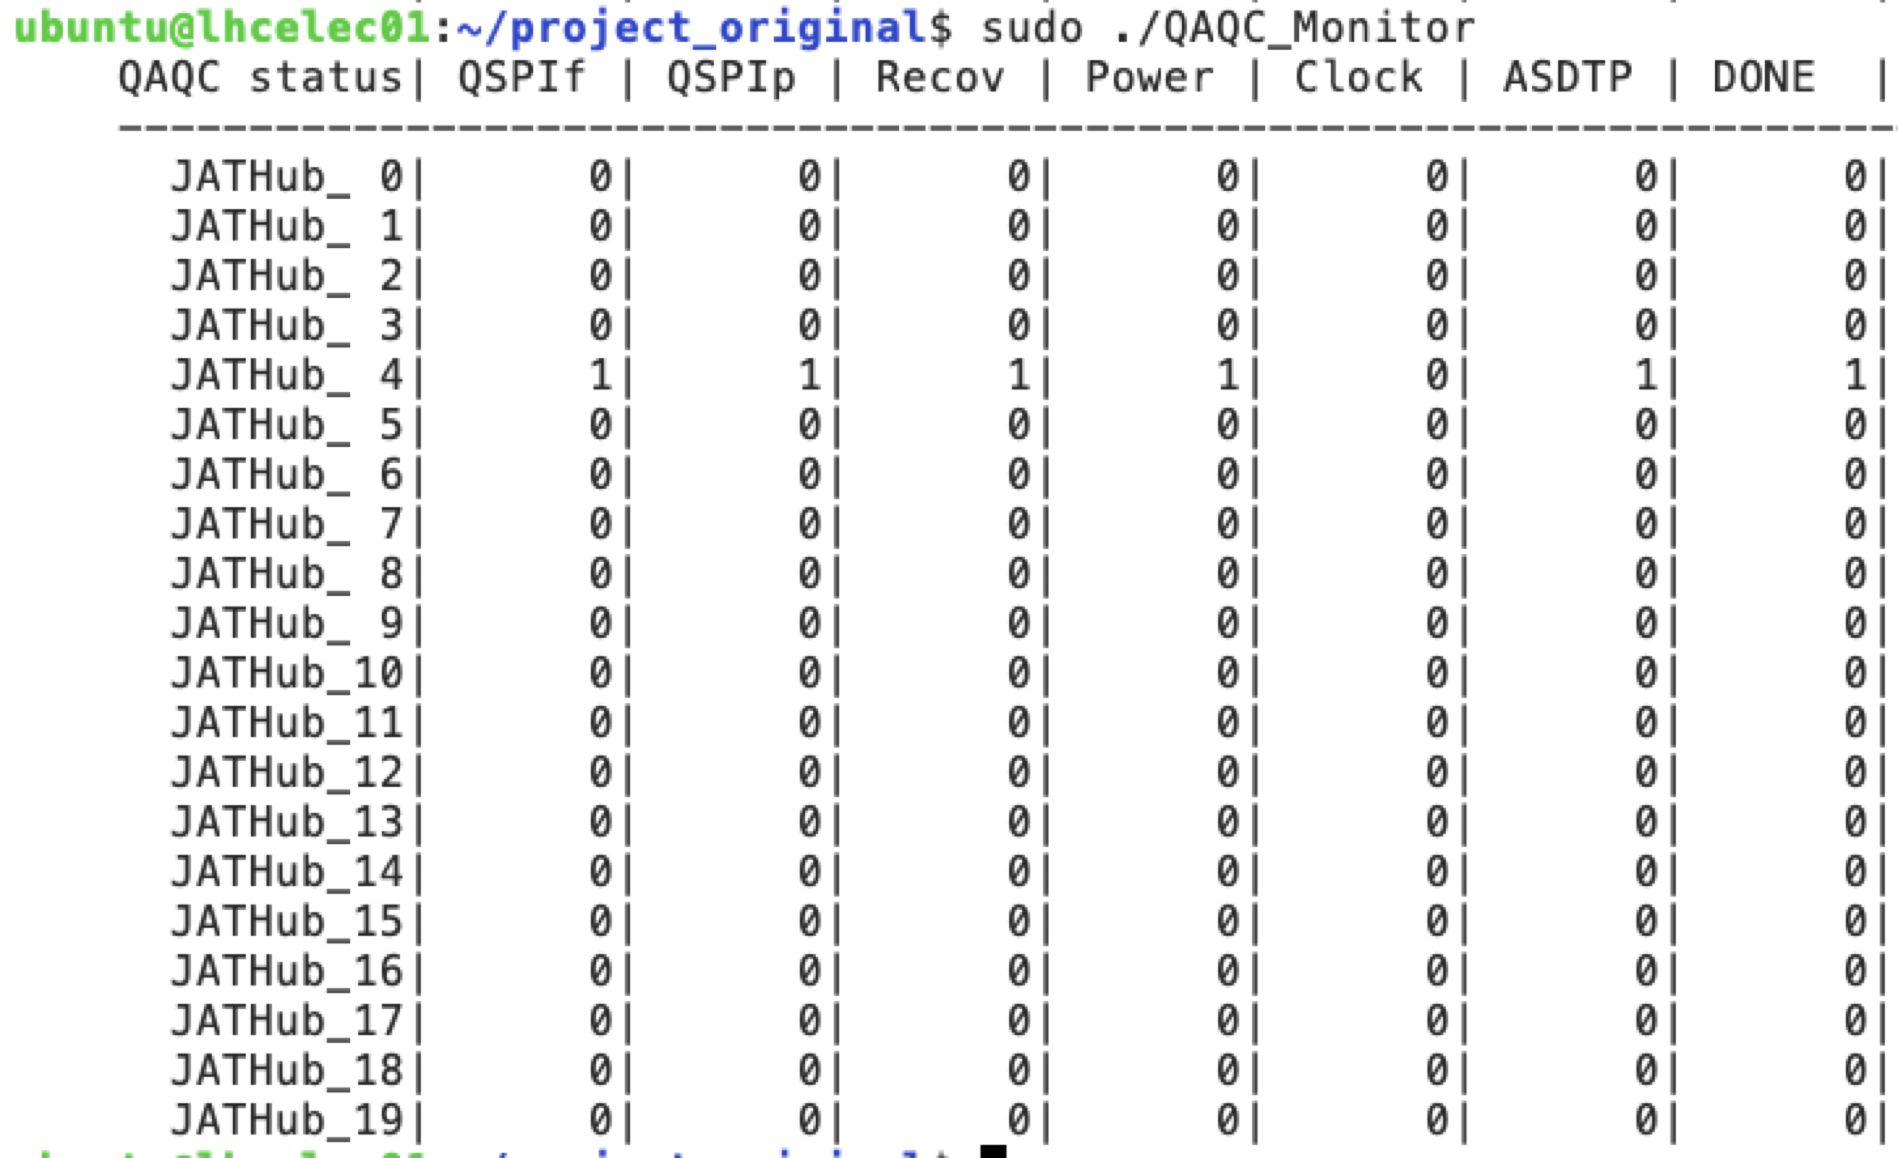
\includegraphics[width=16cm]{fig/QAQC/QAQC_monitor.png}
\caption[JATHubマスターからの試験状況のモニター]{JATHubマスターから試験状況をモニターしている様子。QAQCマスターのスレーブとして動作する20台のJATHubの試験状況をマスターから把握することができる。この写真はQAQC用スレーブ1台を用いた試験の際に取られたものであり、JATHub4がそれに該当する。}
\label{QAQC_monitor}
\end{figure}

\begin{figure} 
\centering
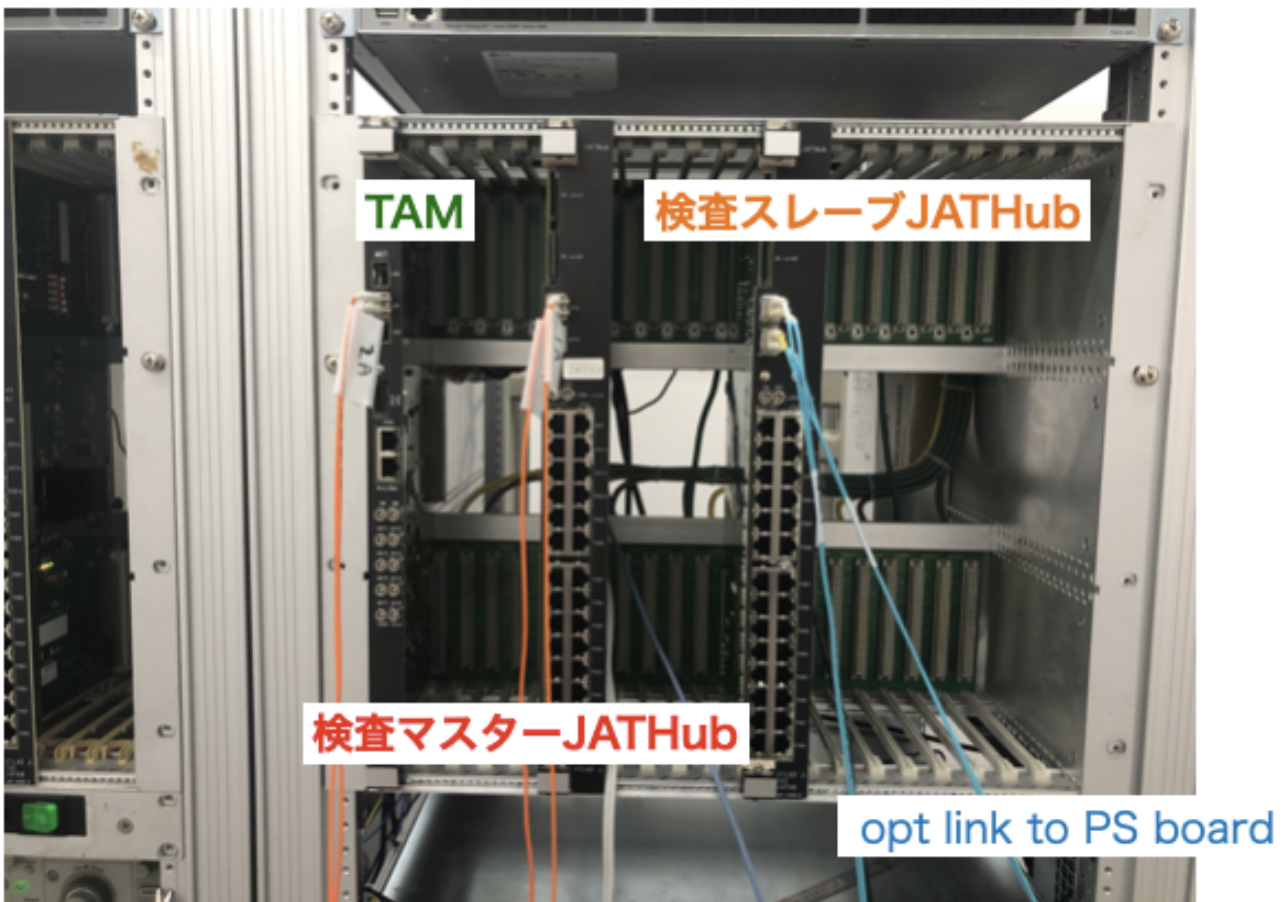
\includegraphics[width=16cm]{fig/QAQC/QAQCpararellpicture.png}
\caption[並列化システムの写真]{並列化システムの写真}
\label{QAQCpararellpicture}
\end{figure}

\section{コンパクトDAQシステムとしての応用例}
\label{sec_compactdaq}
最後に、本研究で開発したQAQC用JATHubの応用例について紹介する。本システムは汎用的なUbuntuをPSに搭載しており拡張性に富んでいることに加え、デスクトップでも給電可能なコンパクトシステムであることからDAQシステムとして幅広い応用が期待される。
実際に使用された例を2つ紹介する。1つ目はEIL4チェンバーの検査試験である。そのときのセットアップを図\ref{JATHubEIL4}に示す。この試験は、高輝度LHC-ATLAS実験に向けて新しく設置されるTGC EIチェンバーの検査を目的としたもので、チェンバーに取り付けたASDからの信号をPS boardで処理し、QAQC用JATHubから読み出している。ASDテストパルスを用いたノイズレートの測定や、セルフトリガー機構を追加実装した上で宇宙線ミューオンを測定する、チャンネルごとのefficiency測定も行われた。
\vskip0.5\baselineskip

\begin{figure}
\centering
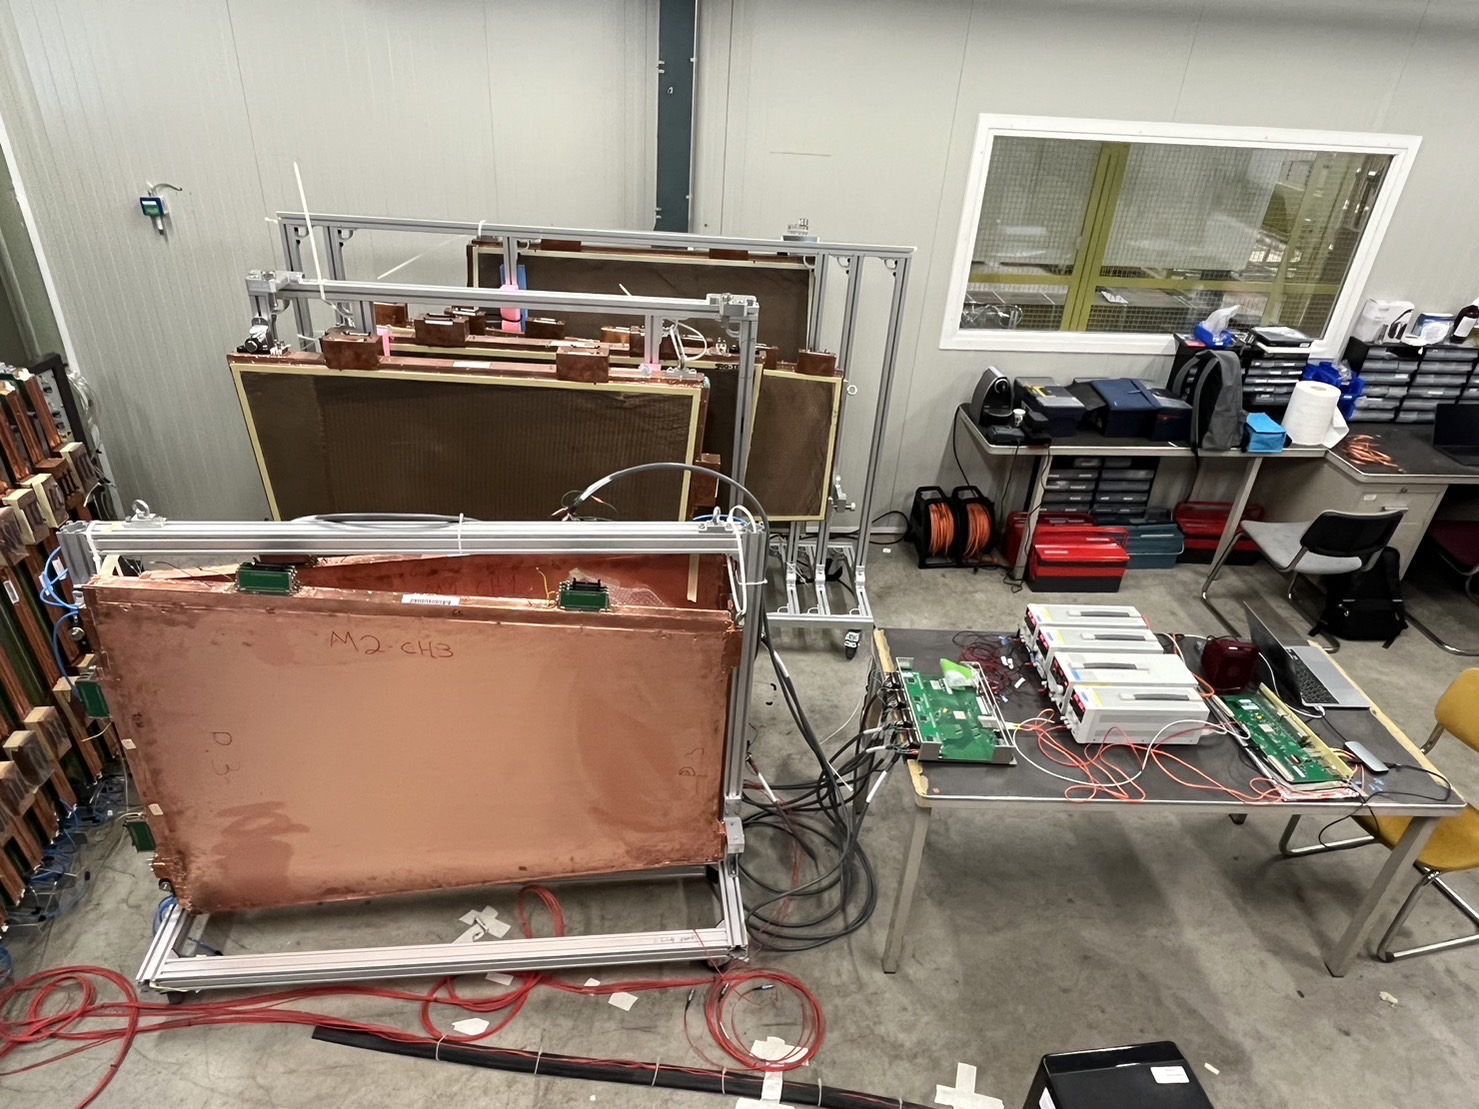
\includegraphics[width=16cm]{fig/QAQC/JATHubEIL4.JPG}
\caption[QAQC用JATHubの使用例:EIL4チェンバー試験]{QAQC用JATHubの使用例:EIL4チェンバー試験\cite{mt_wada}}
\label{JATHubEIL4}
\end{figure}

2つ目はPS baordの放射線耐性試験である(図\ref{JATHubSEU})。この試験は、ATLAS実験室の実際の放射線環境においてPS boardにどれだけSEUが発生するか検証することを目的としたもので、UX15に設置したPS boardから送られるモニターデータの読み出しにQAQC用JATHubは使われている。

\begin{figure}
\centering
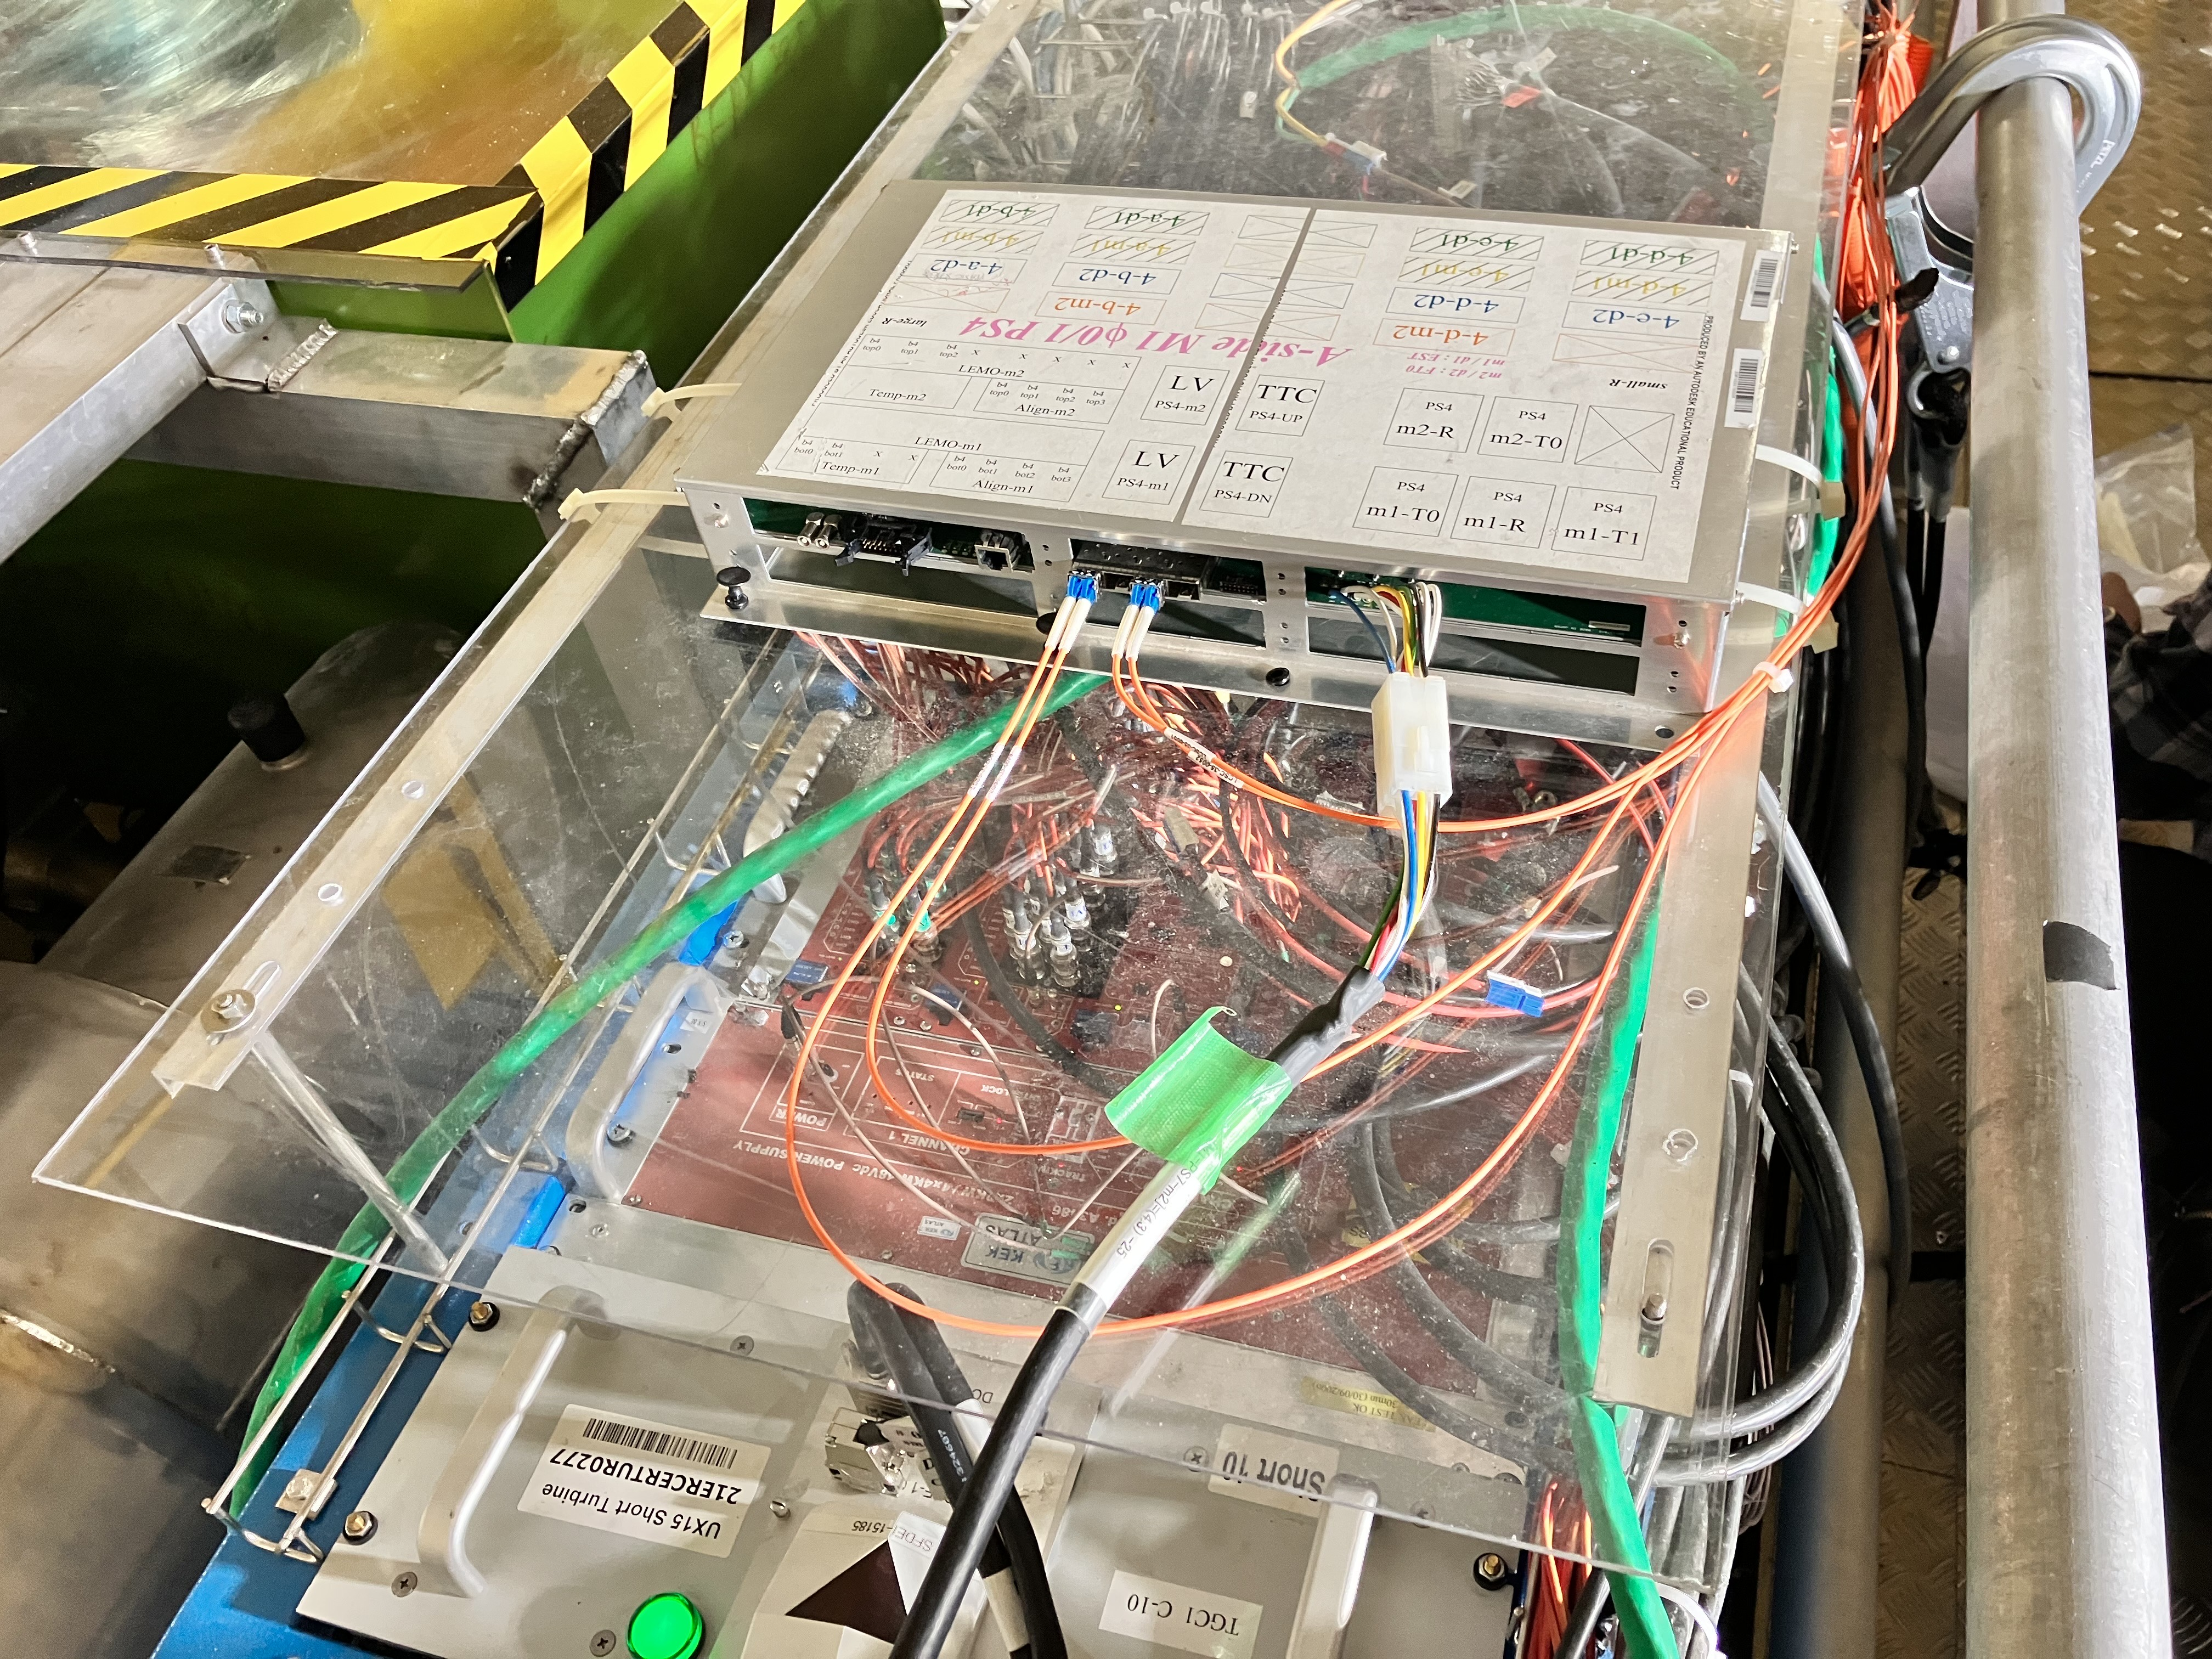
\includegraphics[width=16cm]{fig/QAQC/JATHubSEU.JPG}
\caption[QAQC用JATHubの使用例:PS board SEUモニター]{QAQC用JATHubの使用例:PS board SEUモニター\cite{mt_hashimoto}}
\label{JATHubSEU}
\end{figure}

その他にもTAMモジュールのQAQC試験やPS boardのメンテナンス目的でも本システムは利用されていく予定であり、高輝度LHC-ATLAS実験に向けたTGCエレクトロニクスのアップデートに欠かせない、重要なインフラとして活用されていく。